% !TEX root=./dummy-06.tex

\chapter{双杂化泛函的静态极化率测评}
\label{sec.6.title}

\section{引言}

在上一章中,我们已经了解静态极化率的意义、其物理定义与计算策略、以及精确的理论计算极化率的具体实现方法。我们还注意到,静态极化率是现在机器学习方法在化学中应用的重要标准之一;许多机器学习方法都将静态极化率作为学习目标\cite{Ramakrishnan-Lilienfeld.SD.2014, Gilmer-Dahl.ICML.2017, Faber-Lilienfeld.JCTC.2017, Schuett-Mueller.NIPS.2017, Schuett-Mueller.JCP.2018, Wilkins-Ceriotti.PNAS.2019, Schuett-Gastegger.arXiv.2021, Zhang-Jiang.Elsevier.2023, Zou-Hu.NCS.2023}。作为二维张量,静态极化率是最基本的具有等变性的分子性质之一;因此对它的正确描述也可以验证机器学习网络的等变性、以及确认等变网络参数的有效性\cite{Cohen-Welling.arXiv.2016, Schuett-Gastegger.arXiv.2021, Brandstetter-Welling.arXiv.2022, Geiger-Smidt.arXiv.2022}。同时,作为参数化方法的学习目标,一些分子力学方法也对电子结构方法的极化率精确性有较高的需求\cite{Halgren-Damm.COSB.2001, Baker-Baker.WCMS.2015, Goloviznina-Padua.JCTC.2019, Schauperl-Gilson.CC.2020}。在大数据与 AI for Science 思潮盛行的时代,可信的、大通量高效的、通过精确的电子结构方法计算得到的静态极化率,将会、或已经成为亟待解决的重要需求。

尽管上一章中发展的 FPA 策略、以及其给出的 CCSD(T)/CBS 级别精确的极化率相当重要,但 CCSD(T) 计算消耗仍然十分巨大;若要将极化率计算应用到更大的体系,或者提升精确极化率计算的效率,则需要计算量更小的基组或电子结构方法。密度泛函近似在计算量与精度上,是普遍为计算化学与固体物理应用工作者所接受的方法;它有希望成为解决大量精确计算静态极化率问题的方法。

如第一章所述,双杂化泛函已经在许多化学反应能量与分子性质的测评上,展现出良好的结果。如第三章所述,双杂化泛函的极化率计算尽管相比于杂化泛函更为耗时,但对于 2000 基组大小以内的中等体系是可以接受的,这也契合目前流行的诸多大数据集 20 重原子以内的分子大小\cite{Ruddigkeit-Reymond.JCIM.2012, Ramakrishnan-Lilienfeld.SD.2014, Bowman-Yu.JCP.2022, Zou-Hu.NCS.2023}。因此,双杂化泛函从计算效率上,应可以胜任静态极化率的大规模计算。对于偏重无机小分子与自旋极化分子的 HH132 数据集,Hait 与 Head-Gordon 的测评结果展示了双杂化泛函、特别是 xDH 型泛函在静态极化率计算结果相当精确\cite{Hait-Head-Gordon.PCCP.2018}。

本章将拓展静态极化率测评结果,以更全面地展示密度泛函的精确性、以及如何高效但不失精度地计算静态极化率。在一定的、可容忍的误差范围内,使用合理大小的基组,可以有效地以较小的代价实现极化率的计算;\ref{sec.6.basis-converg} 节将对典型的双杂化泛函,B2PLYP 泛函与 xDH@B3LYP 类型泛函,对于静态极化率问题作基组误差分析,以探讨基组对计算精度的影响。目前基于高精度 CCSD(T)/CBS 精度的测评,仅涉及到少量双杂化泛函以及 HH132\cite{Hait-Head-Gordon.PCCP.2018} 为代表的小型无机分子;\ref{sec.6.benchmark} 节将基于第五章的 CCSD(T)/CBS 精度的参考值,拓展数据集到 HR46\cite{Hickey-Rowley.JPCA.2014} 与 T144\cite{Wu-Thakkar.CPL.2015},测评包括更多双杂化泛函在内的诸密度泛函近似在静态极化率上的表现。对于分子性质的测评,最终应服务于密度泛函的发展;作为最初步的探索,\ref{sec.6.pol-xdh-optimize} 节将基于 xDH@B3LYP 参数化模型\cite{Zhang-Xu.JPCL.2021},仅针对极化率测评表现进行参数优化,探究 xDH@B3LYP 模式在极化率问题上的极限。

\section{实现细节}

本章工作继承第五章工作;大多数实现细节上也参考 \alertref{sec.5.detail} 节。需要额外说明或有所不同的实现细节列出如下。

\subsection{数据集}

本章将测评 HR46\cite{Hickey-Rowley.JPCA.2014} 与 T144\cite{Wu-Thakkar.CPL.2015} 数据集。这两个数据集的 CCSD(T) 方法 FPA-aV[DT]Z、FPA-aV[TQ]Z 或 FPA-aV[Q5]Z 级别下计算得到的同性极化率 $\alpha$、异性极化率 $\gamma$ 的参考值已由表 \alertref{tab.5.s1}, \alertref{tab.5.s2}, \alertref{tab.5.s3}, \alertref{tab.5.s4} 给出。

本章工作也对 HH132 数据集\cite{Hait-Head-Gordon.PCCP.2018}的部分分子作测评与分析。由于诸多原因,HH132 中实际被测评的分子是 75 个自旋非极化分子、以及 26 个自旋极化分子,总共 101 个分子。详细说明见 \ref{sec.6.supp-HH132-remove} 节的讨论。本章后续将称该数据集为 HH101 数据集;对该数据集的误差讨论与分析中,将区分 75 个自旋极化 (SP) 与 26 个自旋非极化分子 (NSP)。该数据集的参考值是 CCSD(T) 方法 aCV[TQ]Z 或 aCV[Q5]Z 计算得到。

\subsection{电子结构计算}

本工作测评的极化率是解析梯度计算得到的结果。程序通过 \textsc{PySCF} (介于 2.1.0 到 2.4.0 版本)以及扩展程序脚本 \textsc{dh} (commit 80ca9e8) 实现。对于所有泛函,DFT 积分所使用的密度格点为第 4 级 (默认修剪、第一周期 (60, 434)、第二周期 (90, 590)、第三周期 (95, 590))。辅助基组均使用 ETB 自动生成基组。在极化率测评中,基组统一使用 aug-pc-3;在基组误差分析中,我们将使用 aCV$X$Z ($X = \mathrm{D, T, Q, 5}$) 与 aug-pc-$n$ ($n = 1, 2, 3, 4$) 基组;所使用到的 CBS 模型与 \alertref{sec.5.cbs} 节相同,且 CBS 外推仅针对相关贡献部分、而对自洽场部分不作外推。后续文段中,我们将简记基组 aug-pc-$n$ 为 apc$n$ ($n = 1, 2, 3, 4$)。

本工作测评并汇报 62 个密度泛函近似的极化率误差结果。被测评泛函分布如图 \ref{fig.6.pol-functionals-distribution} 所示。我们尽可能对目前流行的、且在 \textsc{dh} 程序中实现的双杂化泛函做极化率测评;涉及到 B95 的双杂化泛函由于部分体系存在收敛问题,本工作暂不纳入 \textsc{dh} 程序已经实现的 DSD-PBEB95-D3BJ 与 PWPB95-D3Zero 泛函;对于 ωB97X-2 泛函,我们仅测评其 TQZ 版本。本工作所涉及到的低阶泛函包括
\begin{itemize}[nosep]
    \item mBEEF, MVS, SCAN, MPW1K, PBE50, SCAN0, MPW91, N12 等泛函是 Hait 与 Head-Gordon 测评工作\cite{Hait-Head-Gordon.PCCP.2018}中表现较好的 GGA 或 mGGA 泛函;
    \item M11, M06-2X 是 T145 测评工作\cite{Wu-Thakkar.CPL.2015}中表现较好的泛函;
    \item PBE, BLYP, TPSS, N12, M06-L, B3LYP, PBE0, M06, TPSSh, MN15, CAM-B3LYP, ωB97M-V 等泛函是目前计算化学应用的常见泛函。
\end{itemize}
对于 ωB97M-V 泛函,本工作的计算不考虑其 VV10 贡献项。

我们同时对 HF、MP2、CCSD 的极化率表现作测评。对于 HH101 数据集,计算结果取自 Hait 与 Head-Gordon 的工作的 aCV[TQ]Z 或 aCV[Q5]Z 计算结果。对于 HR46 与 T144 数据集,计算结果取自第五章工作;即 HF 与 MP2 使用 aCV[Q5]Z 计算结果,CCSD 使用 FPA-aV[DT]Z、FPA-aV[TQ]Z 或 FPA-aV[Q5]Z 计算结果。

\subsection{误差测评标准}

对于同性极化率 $\alpha$、异性极化率 $\gamma$ 的计算,我们将沿用式 \alertref{eq.5.relrmsd} 的 RelRMSD 误差量标。对于 HH101 数据集的测评,我们也对其极化率分量使用 RelRMSD 量标\footnote{HH132 原始文献\cite{Hait-Head-Gordon.PCCP.2018}中,Hait 等提出的误差量标是 RMSRE;若 RelRMSD 表达式 \alertref{eq.5.relrmsd} 的指标 $n$ 代表的不是分子、而是分子极化率的 $\alpha_{xx}, \alpha_{yy}, \alpha_{zz}$ 分量之一,那么 HH132 原始文献式 (3) 所表达的 RMSRE 与本工作的 RelRMSD 是等价的。但需要注意到,在 HH132 文献的 Supporting Information 中,Hait 等实际计算与汇报的误差是三个分量的平均值、而非方均根平均;即以 HH132 原始文献的记号,
$$
\text{RMSRE (reported)} = \frac{1}{3} \sum_{i=x,y,z} \sqrt{\frac{1}{N} \sum_{n=1}^N \varepsilon_{i,n}^2}
$$
这与 HH132 原文献的式 (3) 表述的方式有所不同;式 (3) 的具体表述是
\begin{equation}
    \label{eq.6.rmsre}
    \text{RMSRE (designed)} = \sqrt{\frac{1}{3N} \sum_{i=x,y,z} \sum_{n=1}^N \varepsilon_{i,n}^2}
\end{equation}
尽管一般来说两者数值上非常接近、且几乎不会影响泛函测评表现。在本工作中,我们使用 HH132 原文献式 (3) 的表述、或者等价地使用 RelRMSD 对数据集的极化率分量 $\alpha_{xx}, \alpha_{yy}, \alpha_{zz}$ 作测评。
}。

由于我们将测评多种数据集以及多种类型的极化率;为简化分析,这里定义加权相对误差 WTRE (\underline{w}eigh\underline{t}ed \underline{r}elative \underline{e}rror) 以对泛函的总体极化率误差进行合适的排序。对于数据集以及其对应的测评性质 $d$,泛函 $f$ 的相对方均根误差 RelRMSD 的测评结果 $\epsilon_{f,d}$,泛函的加权相对误差是
\begin{equation}
    \label{eq.6.wtre}
    \mathrm{WTRE}_f = \sum_d w_d \epsilon_{f,d}
\end{equation}
具体的测评性质 $d$、以及权重 $w_d$ 定义如表 \ref{tab.6.benchmark-weight} 所示。WTRE 是无量纲量,也并非百分比误差。权重 $w_d$ 定义为反比于本工作所测评泛函的平均 RelRMSD 误差的量:
\begin{equation}
    w_d = \frac{1}{\mathrm{count} \{ d \}} \frac{1}{\mathrm{count} \{ f \}} \frac{1}{\displaystyle \sum_{f} \epsilon_{f,d}}
\end{equation}
其中,$\mathrm{count} \{ d \} = 8$ 是指 8 个被测评的性质 (参考表 \ref{tab.6.benchmark-weight}),$\mathrm{count} \{ f \}$ 是指被测评的 64 个泛函 (参考图 \ref{fig.6.pol-functionals-distribution})。在此定义下,本工作所测评的泛函 WTRE 误差的平均值是 1,即
\begin{equation*}
    \frac{1}{\mathrm{count} \{ f \}} \sum_f \mathrm{WTRE}_f = 1
\end{equation*}
若泛函 $f$ 所对应的加权误差 $\mathrm{WTRE}_f$ 越小,则泛函 $f$ 的总体极化率表现越好;若 $\mathrm{WTRE}_f$ 接近 1,则表明泛函 $f$ 的测评表现处于平均水平。

\begin{figure}[t]
    \centering
    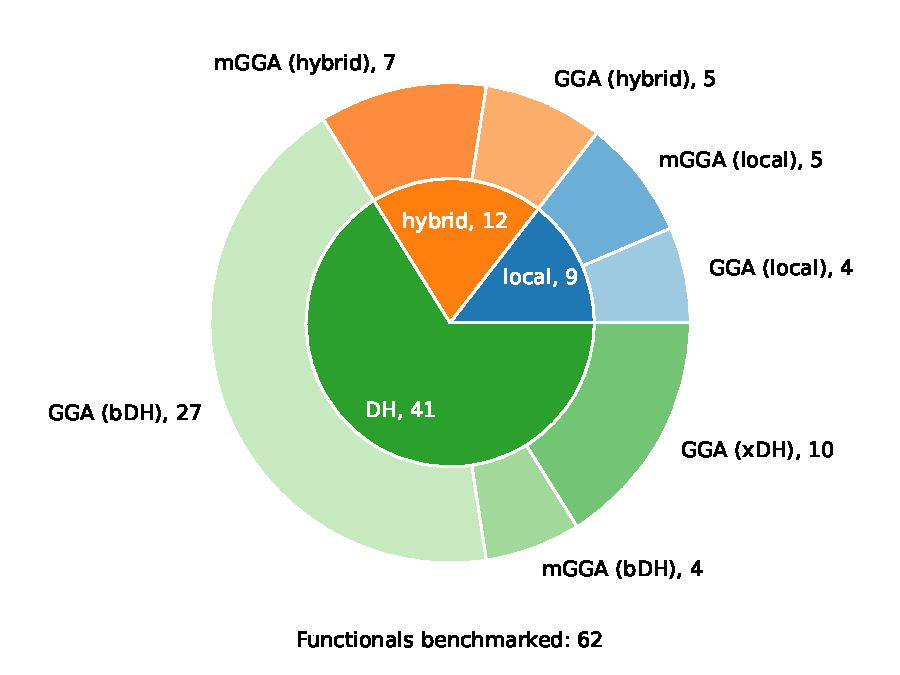
\includegraphics[width=0.6\textwidth]{assets/pol-functionals-distribution.pdf}
    \caption{本工作测评泛函的大致分类与数量示意图。}
    \label{fig.6.pol-functionals-distribution}
\end{figure}

\begin{table}[!ht]
\centering
\caption{极化率测评权重表。}
\label{tab.6.benchmark-weight}
\widetabular{
    \begin{tabular}{lld{3.8}}
    \toprule
    性质        & 数据集 ($d$) & \multicolumn{1}{c}{权重 ($w_d$)} \\ \midrule
    同性极化率  & HR46        & 0.0618371 \\
                & T144        & 0.0548781 \\
                & HH101 (NSP) & 0.0382151 \\
                & HH101 (SP)  & 0.0326924 \\ \midrule
    异性极化率\tnote{a} & HR46        & 0.0245850 \\
                & T144        & 0.0250915 \\ \midrule
    极化率分量  & HH101 (NSP) & 0.0370998 \\
                & HH101 (SP)  & 0.0298901 \\ \bottomrule
    \end{tabular}
}{
    \item[a] 部分分子异向极化率 $\gamma$ 小于 0.5 \AA${}^3$,不适合作相对误差分析;因此对于异向极化率,HR46 数据集总共测评 39 个分子 (除去 \ce{H2O}, \ce{CH4}, \ce{CH3F}, \ce{PH2}, \ce{H2S}, \ce{SiH4}, \ce{NH3} 共七个分子),T144 数据集总共测评 141 个分子 (除去 0351 \ce{C2H5F}, 0353 \ce{CH3F}, 0998 \ce{CF3CHF2} 共三个分子)。
}
\end{table}

\subsection{泛函参数优化}

本工作将会简要地考察泛函的参数调整问题。我们选用 \textsc{SciPy}\cite{Virtanen-Vazquez-Baeza.NM.2020} 进行泛函参数的优化。优化算法选用 L-BFGS-B 算法\cite{Byrd-Zhu.SJSC.1995},收敛判标是参数梯度模长 (\verb|gtol|) 小于 $10^{-5}$。我们采用简单的全局优化方法,即在优化后的泛函参数上施加不超过 0.5 的随机参数系数再次优化,反复 20 次,并汇报取得最低 $\mathrm{WTRE}_f$ 时的泛函参数。

\section{典型双杂化泛函静态极化率基组误差分析}
\label{sec.6.basis-converg}

这一节中,我们将以典型的双杂化泛函 B2PLYP 作为例子,分析其静态极化率的基组误差。

对于 B2PLYP 而言,其同性极化率 $\alpha_\textsf{DH}$ 可以分解为自洽场部分 $\alpha_\textsf{SCF}$ 与二阶微扰部分 $\symup{\Delta} \alpha_\textsf{PT}$ 之和
\begin{equation*}
    \alpha_\textsf{DH} = \alpha_\textsf{SCF} + \symup{\Delta} \alpha_\textsf{PT2} \quad \text{(B2PLYP-like doubly hybrid)}
\end{equation*}
我们将对这两部分分量,分别作基组收敛分析。作为基准,我们选取 aCV[Q5]Z 的 CBS 外推模型作为参考值;这也与第五章的最佳 CBS 外推标准相同:
\begin{equation*}
    \alpha_\textsf{DH} (\text{aCV[Q5]Z}) = \alpha_\textsf{SCF} (\text{aCV5Z}) + \symup{\Delta} \alpha_\textsf{PT2} (\text{aCV[Q5]Z})
\end{equation*}
对于其他 CBS 外推模式下的双杂化泛函极化率,其自洽场部分将使用较大的基组结果、而二阶微扰部分将采用 CBS 外推:
\begin{align*}
    \alpha_\textsf{DH} (\text{aCV}[XY]\text{Z}) &= \alpha_\textsf{SCF} (\text{aCV}Y\text{Z}) + \symup{\Delta} \alpha_\textsf{PT2} (\text{aCV}[XY]\text{Z}) \; &&([XY] = \mathrm{[DT], [TQ]}) \\
    \alpha_\textsf{DH} (\text{apc}[nm]) &= \alpha_\textsf{SCF} (\text{apc}m) + \symup{\Delta} \alpha_\textsf{PT2} (\text{apc}[nm]) \; &&([nm] = [12], [23], [34])
\end{align*}
对于异性极化率 $\gamma_\textsf{DH}$ 也可以作类似的拆解。

\subsection{HR46 与 T144 数据集分析}

HR46 与 T144 大多数分子为有机分子、且分子大小较大,两个数据集较为相近。表 \ref{tab.6.b2p-conv-hr46-t144-iso} 与表 \ref{tab.6.b2p-conv-hr46-t144-aniso} 分别展示了 HR46 与 T144 数据集下 B2PLYP 在同性极化率 $\alpha$ 与异性极化率 $\gamma$ 下的基组收敛性表现。

\begin{table}[!ht]
\centering
\caption{B2PLYP 在数据集 HR46 与 T144 下同性极化率 $\alpha$ 的基组相对方均根误差 (RelRMSD / \%)${}^a$。}
\label{tab.6.b2p-conv-hr46-t144-iso}
\widetabular{
    \begin{tabular}{cld{1.3}d{1.3}d{1.3}d{1.3}d{1.3}d{1.3}}
    \toprule
    & & \multicolumn{3}{c}{HR46} & \multicolumn{3}{c}{T144} \\
    \cmidrule(lr){3-5} \cmidrule(lr){6-8}
    基组基数 & 基组 & \multicolumn{1}{c}{$\tilde \alpha_\textsf{SCF}$\tnote{b}} & \multicolumn{1}{c}{$\symup{\Delta} \tilde \alpha_\textsf{PT2}$\tnote{c}} & \multicolumn{1}{c}{$\tilde \alpha_\textsf{DH}$\tnote{d}} & \multicolumn{1}{c}{$\tilde \alpha_\textsf{SCF}$} & \multicolumn{1}{c}{$\symup{\Delta} \tilde \alpha_\textsf{PT2}$} & \multicolumn{1}{c}{$\tilde \alpha_\textsf{DH}$} \\
    \midrule
    2-$\zeta$ & aCVDZ    & 2.428 & 0.250 & 2.528 & 1.560 & 0.185 & 1.448 \\
              & apc1     & 1.001 & 0.188 & 0.905 & 0.855 & 0.225 & 0.686 \\ \midrule
    3-$\zeta$ & aCVTZ    & 0.542 & 0.120 & 0.571 & 0.241 & 0.134 & 0.152 \\
              & apc2     & 0.262 & 0.144 & 0.187 & 0.222 & 0.166 & 0.099 \\
              & aCV[DT]Z &       & 0.111 & 0.532 &       & 0.124 & 0.146 \\
              & apc[12]  &       & 0.153 & 0.224 &       & 0.150 & 0.114 \\ \midrule
    4-$\zeta$ & aCVQZ    & 0.086 & 0.069 & 0.121 & 0.018 & 0.082 & 0.073 \\
              & apc3     & 0.067 & 0.061 & 0.120 & 0.029 & 0.078 & 0.104 \\
              & aCV[TQ]Z &       & 0.057 & 0.096 &       & 0.049 & 0.041 \\
              & apc[23]  &       & 0.029 & 0.073 &       & 0.019 & 0.044 \\ \midrule
    5-$\zeta$ & aCV5Z    & \multicolumn{1}{c}{0\tnote{e}} & 0.036 & 0.036 & \multicolumn{1}{c}{0\tnote{e}} & 0.042 & 0.042 \\
              & apc4     & 0.099 & 0.046 & 0.140 & 0.050 & 0.054 & 0.102 \\
              & aCV[Q5]Z &       & \multicolumn{1}{c}{0\tnote{e}} & \multicolumn{1}{c}{0\tnote{e}} &       & \multicolumn{1}{c}{0\tnote{e}} & \multicolumn{1}{c}{0\tnote{e}} \\
              & apc[34]  &       & 0.034 & 0.127 &       & 0.032 & 0.080 \\
    \bottomrule
    \end{tabular}
}{
    \item[a] 该表格的部分数值因为选取为参考值,因此 $\tilde \alpha_\textsf{SCF}$ 在 aCV5Z、$\symup{\Delta} \tilde \alpha_\textsf{PT2}$ 与 $\tilde \alpha_\textsf{DH}$ 在 aCV[Q5]Z 下的误差值严格为零。
    \item[b] 自洽场部分同性极化率相对方均根误差为 $\text{RelRMSD} (\tilde \alpha_{\textsf{SCF}/\text{basis}}, \tilde \alpha_{\textsf{SCF}/\text{ref}}, \tilde \alpha_{\textsf{DH}/\text{ref}})$。其中,$\tilde \alpha_{\textsf{SCF}/\text{ref}}$ 指代的是大基组的 $\tilde \alpha_{\textsf{SCF}/\text{aCV5Z}}$,$\tilde \alpha_{\textsf{DH}/\text{ref}}$ 指代的是作为大基组参考值的 $\tilde \alpha_{\textsf{DH}/\text{aCV[Q5]Z}}$。
    \item[c] 二阶微扰部分同性极化率相对方均根误差为 $\text{RelRMSD} (\symup{\Delta} \tilde \alpha_{\textsf{PT2}/\text{basis}}, \symup{\Delta} \tilde \alpha_{\textsf{PT2}/\text{ref}}, \tilde \alpha_{\textsf{DH}/\text{ref}})$。其中,$\symup{\Delta} \tilde \alpha_{\textsf{PT2}/\text{ref}}$ 指代的是大基组的 $\symup{\Delta} \tilde \alpha_{\textsf{PT2}/\text{aCV[Q5]Z}}$。
    \item[d] 双杂化总同性极化率相对方均根误差为 $\text{RelRMSD} (\tilde \alpha_{\textsf{DH}/\text{basis}}, \tilde \alpha_{\textsf{DH}/\text{ref}})$。
    \item[e] 这些数值依据参考值的选取方式,从定义上是零。
}
\end{table}

\begin{table}[!ht]
\centering
\caption{B2PLYP 在数据集 HR46 与 T144 下异性极化率 $\gamma$ 的基组相对方均根误差 (RelRMSD / \%)${}^a$。}
\label{tab.6.b2p-conv-hr46-t144-aniso}
\widetabular{
    \begin{tabular}{cld{1.3}d{1.3}d{1.3}d{1.3}d{1.3}d{1.3}}
    \toprule
    & & \multicolumn{3}{c}{HR46} & \multicolumn{3}{c}{T144} \\
    \cmidrule(lr){3-5} \cmidrule(lr){6-8}
    基组基数 & 基组 & \multicolumn{1}{c}{$\tilde \gamma_\textsf{SCF}$} & \multicolumn{1}{c}{$\symup{\Delta} \tilde \gamma_\textsf{PT2}$} & \multicolumn{1}{c}{$\tilde \gamma_\textsf{DH}$} & \multicolumn{1}{c}{$\tilde \gamma_\textsf{SCF}$} & \multicolumn{1}{c}{$\symup{\Delta} \tilde \gamma_\textsf{PT2}$} & \multicolumn{1}{c}{$\tilde \gamma_\textsf{DH}$} \\
    \midrule
    2-$\zeta$ & aCVDZ    & 3.389 & 0.505 & 3.596 & 1.742 & 0.264 & 1.860 \\
              & apc1     & 2.271 & 0.892 & 2.885 & 1.321 & 0.446 & 1.530 \\ \midrule
    3-$\zeta$ & aCVTZ    & 0.777 & 0.122 & 0.845 & 0.313 & 0.090 & 0.374 \\
              & apc2     & 0.342 & 0.311 & 0.503 & 0.159 & 0.145 & 0.201 \\
              & aCV[DT]Z &       & 0.230 & 0.845 &       & 0.137 & 0.383 \\
              & apc[12]  &       & 0.130 & 0.351 &       & 0.103 & 0.170 \\ \midrule
    4-$\zeta$ & aCVQZ    & 0.140 & 0.073 & 0.196 & 0.053 & 0.059 & 0.090 \\
              & apc3     & 0.102 & 0.124 & 0.174 & 0.061 & 0.058 & 0.085 \\
              & aCV[TQ]Z &       & 0.058 & 0.183 &       & 0.043 & 0.079 \\
              & apc[23]  &       & 0.099 & 0.115 &       & 0.050 & 0.055 \\ \midrule
    5-$\zeta$ & aCV5Z    & \multicolumn{1}{c}{0} & 0.038 & 0.038 & \multicolumn{1}{c}{0} & 0.030 & 0.030 \\
              & apc4     & 0.108 & 0.053 & 0.130 & 0.061 & 0.038 & 0.073 \\
              & aCV[Q5]Z &       & \multicolumn{1}{c}{0} & \multicolumn{1}{c}{0} &       & \multicolumn{1}{c}{0} & \multicolumn{1}{c}{0} \\
              & apc[34]  &       & 0.041 & 0.122 &       & 0.037 & 0.071 \\
    \bottomrule
    \end{tabular}
}{
    \item[a] 该表格的图例参考表 \ref{tab.6.b2p-conv-hr46-t144-iso}。
}
\end{table}

可以看到,若不考虑计算量相当大的 5-$\zeta$ 基组或 CBS 方法,对于双杂化泛函总极化率 $\alpha_\textsf{DH}$ 或 $\gamma_\textsf{DH}$,Jensen 基组 apc$n$ ($n = 1, 2, 3$) 通常比 Dunning 基组 aCV$X$Z ($X = \mathrm{D, T, Q}$) 在相同的基组基数 $\zeta$ 下,有更低的误差 (例外是 T144 数据集 4-$\zeta$ 下同性极化率 $\alpha_\textsf{DH}$ 的相对方均根误差)。而同时注意到,对于相同的基组基数 $\zeta$,Jensen 基组 apc$n$ 的大小通常小于 Dunning 基组 aCV$X$Z;因此对于 2,3,4-$\zeta$ 的情形,Jensen 基组 apc$n$ 在极化率计算问题上,不论是性能需求还是误差都要好于 Dunning 基组 aCV$X$Z。

在 \alertref{sec.5.bench-wft-polar} 小节对小分子体系 MP2 极化率的基组误差分析中,HF 方法的极化率 $\alpha_\textsf{HF}$ 与 $\gamma_\textsf{HF}$ 的误差,随着基组基数 $\zeta$ 的增大而快速减小。而相对地,MP2 的相关贡献 $\symup{\Delta} \alpha_\textsf{(2)}$ 与 $\symup{\Delta} \gamma_\textsf{(2)}$ 的收敛趋势较慢;对于同性极化率 $\symup{\Delta} \alpha_\textsf{(2)}$ 的误差在 4,5-$\zeta$ 下远远大于 $\alpha_\textsf{HF}$。而对于 HR46 与 T144 数据集的 B2PLYP 计算下,二阶微扰贡献 $\symup{\Delta} \alpha_\textsf{PT2}$ 与 $\symup{\Delta} \gamma_\textsf{PT2}$ 的误差相比于自洽场部分 $\alpha_\textsf{SCF}$ 与 $\gamma_\textsf{SCF}$ 一般来说相当或更小。注意到 B2PLYP 泛函的二阶微扰贡献系数 $c_\mathrm{c} = 0.27$,因此尽管二阶微扰本身的收敛趋势较慢、但在系数的缩放下并没有体现出很大的误差。

对于 Jensen 基组 apc$n$,其计算同性极化率 $\alpha_\textsf{DH}$ 时,apc2 的误差已经小于 0.2\%;甚至在 T144 数据集下 $\alpha_\textsf{DH}$ 的相对方均根误差为 0.099\%,比之计算代价更大的 apc3 基组的误差更小。但同时考虑到构成 $\alpha_\textsf{DH}$ 的两个分项 $\alpha_\textsf{SCF}$ 与 $\symup{\Delta} \alpha_\textsf{PT2}$,apc2 在这两个分项的误差远远大于 apc3。因此,apc2 同性极化率 $\alpha_\textsf{DH}$ 相当小的误差,应当归因于 $\alpha_\textsf{SCF}$ 与 $\symup{\Delta} \alpha_\textsf{PT2}$ 误差的相互抵消,而不应认为其同性极化率 $\alpha_\textsf{DH}$ 已经接近基组极限;考虑到其他双杂化泛函的构造与 B2PLYP 有所不同,apc2 的 $\alpha_\textsf{DH}$ 计算结果未必能保证对 B2PLYP 以外的其他双杂化泛函有稳定的低误差。

CBS 外推模型在 4-$\zeta$ 的基组基数下有较好的效果:相对于单一基组 aCVQZ 或 apc3 计算,CBS 外推的 aCV[TQ]Z 或 apc[23] 的误差有所降低。对于 3-$\zeta$ 下,CBS 外推与否对同性极化率 $\symup{\Delta} \alpha_\textsf{PT2}$ 影响较小;而对异性极化率 $\symup{\Delta} \gamma_\textsf{PT2}$,Dunning 基组 aCV[DT]Z 的误差比 aCVTZ 误差大、但 Jensen 基组 apc[12] 的误差比 apc2 小。值得注意的是,apc[12] 的同性极化率误差比 $\symup{\Delta} \alpha_\textsf{PT2}$ 小、但 $\alpha_\textsf{DH}$ 的误差反而更大;即每个极化率贡献项分别更小的误差,反而在总和的结果上给出更大的误差;这也印证了 apc2 较低的 $\alpha_\textsf{DH}$ 误差不能表明 apc2 本身的误差很小。

尽管 CBS 外推模型在 4-$\zeta$ 基组基数有良好表现,但注意到 4-$\zeta$ 基组 aCVQZ、apc3 本身的计算误差也仅有不到 0.2\%,CBS 外推的优势比较有限。因此,我们认为对于 HR46 与 T144 数据集,使用 4-$\zeta$ 基组 aCVQZ、apc3 进行双杂化泛函的计算,误差较低且远低于实验误差的 0.5\%,是适合用于测评的基组。而对于 3-$\zeta$,若分别考察 $\alpha_\textsf{SCF}$ 与 $\symup{\Delta} \alpha_\textsf{PT2}$ 分别的误差并作加和,则对于 HR46 数据集的 aCVTZ 或 aCV[DT]Z 误差在 0.65\% 左右,HR46 数据集的 apc2 或 apc[12]、以及 T144 数据集的 3-$\zeta$ 基组或 CBS 外推模型的误差在 0.40\% 左右。apc2 或 apc[12] 的误差尽管小于实验误差的 0.5\%,但幅度不是很大。我们认为,apc2 或 apc[12] 也是可以接受的;但在计算量可接受的情形下,应尽可能使用 4-$\zeta$ 基组或 CBS 外推模型。

最后,我们指出,表 \ref{tab.6.b2p-conv-hr46-t144-iso} 与表 \ref{tab.6.b2p-conv-hr46-t144-aniso} 的数据将表明 5-$\zeta$ 情形下 Jensen 基组 apc4 与 apc[34] 的误差普遍比 Dunning 基组 aCV5Z 更大;并且尽管 apc4 与 apc[34] 计算代价更大,其误差并未比 apc3 与 apc[23] 更进步、甚至误差更大。对此,我们认为,5-$\zeta$ 情形下 Jensen 基组与 Dunning 基组之间的误差反映的是 5-$\zeta$ 级别基组的基组不完备程度;这个不完备程度一般小于 0.2\%,且远小于 0.5\% 的实验误差,这是完全可以接受的误差范围。除此之外,这里作 B2PLYP 基组误差分析的目的,是确认一种在可接受误差的前提下计算效率更高的基组、以及确定基组误差对双杂化泛函测评的影响;当基组达到 4-$\zeta$ 或更大时,其极化率相对误差已经远小于 0.5\%,不会对泛函测评的结果产生明显影响。关于 5-$\zeta$ 级别基组或 CBS 外推方法精度的更多分析,我们在附录 \ref{sec.6.supp-bsie} 小节中展开。

\subsection{HH101 数据集分析}

HH101 数据集包含的分子或原子较小、且有机分子很少;其数据集构成与 HR46 与 T144 有较大差异。表 \ref{tab.6.b2p-conv-hh101-iso} 展示了 HH101 数据集下 B2PLYP 在同性极化率 $\alpha$ 下的基组收敛性表现。

\begin{table}[!ht]
\centering
\caption{B2PLYP 在数据集 HH101 下同性极化率 $\alpha$ 的基组相对方均根误差 (RelRMSD / \%)${}^a$。}
\label{tab.6.b2p-conv-hh101-iso}
\widetabular{
    \begin{tabular}{cld{1.3}d{1.3}d{1.3}d{1.3}d{1.3}d{1.3}}
    \toprule
    & & \multicolumn{3}{c}{HH101 (NSP)\tnote{b}} & \multicolumn{3}{c}{HH101 (SP)} \\
    \cmidrule(lr){3-5} \cmidrule(lr){6-8}
    基组基数 & 基组 & \multicolumn{1}{c}{$\tilde \alpha_\textsf{SCF}$} & \multicolumn{1}{c}{$\symup{\Delta} \tilde \alpha_\textsf{PT2}$} & \multicolumn{1}{c}{$\tilde \alpha_\textsf{DH}$} & \multicolumn{1}{c}{$\tilde \alpha_\textsf{SCF}$} & \multicolumn{1}{c}{$\symup{\Delta} \tilde \alpha_\textsf{PT2}$} & \multicolumn{1}{c}{$\tilde \alpha_\textsf{DH}$} \\
    \midrule
    2-$\zeta$ & aCVDZ    & 4.565 & 0.569 & 4.939 & 3.721 & 0.746 & 4.030 \\
              & apc1     & 1.783 & 0.882 & 1.991 & 1.642 & 0.944 & 1.800 \\ \midrule
    3-$\zeta$ & aCVTZ    & 1.358 & 0.294 & 1.568 & 0.866 & 0.325 & 1.006 \\
              & apc2     & 0.508 & 0.334 & 0.450 & 0.622 & 0.618 & 0.693 \\
              & aCV[DT]Z &       & 0.218 & 1.469 &       & 0.213 & 0.916 \\
              & apc[12]  &       & 0.550 & 0.578 &       & 0.500 & 0.605 \\ \midrule
    4-$\zeta$ & aCVQZ    & 0.302 & 0.150 & 0.432 & 0.146 & 0.205 & 0.282 \\
              & apc3     & 0.196 & 0.109 & 0.248 & 0.167 & 0.143 & 0.190 \\
              & aCV[TQ]Z &       & 0.070 & 0.344 &       & 0.161 & 0.219 \\
              & apc[23]  &       & 0.257 & 0.329 &       & 0.224 & 0.344 \\ \midrule
    5-$\zeta$ & aCV5Z    & \multicolumn{1}{c}{0} & 0.077 & 0.077 & \multicolumn{1}{c}{0} & 0.105 & 0.105 \\
              & apc4     & 0.216 & 0.075 & 0.256 & 0.136 & 0.112 & 0.190 \\
              & aCV[Q5]Z &       & \multicolumn{1}{c}{0} & \multicolumn{1}{c}{0} &       & \multicolumn{1}{c}{0} & \multicolumn{1}{c}{0} \\
              & apc[34]  &       & 0.155 & 0.283 &       & 0.094 & 0.177 \\
    \bottomrule
    \end{tabular}
}{
    \item[a] 该表格的图例参考表 \ref{tab.6.b2p-conv-hr46-t144-iso}。
    \item[b] 由于氢原子在 \textsc{dh} 程序中无法给出解析极化率,因此分析自旋非极化分子总体误差时排除氢原子,即总共分析 74 个自旋非极化体系。
}
\end{table}

可以看到,在相同的基组大小下,HH101 数据集的基组误差相比于 HR46 或 T144 数据集有更大的误差。以 4-$\zeta$ 级别基组来看,HR46 与 T144 数据集同性极化率对于 aCVQZ 与 apc3、以及对应的 CBS 外推模型下,$\alpha_\textsf{SCF}$ 与 $\symup{\Delta} \alpha_\textsf{PT2}$ 的相对方均根误差之和普遍 0.15\% 以内;但在 HH101 数据集中,aCVQZ 在自旋非极化的 74 个分子中,其 $\alpha_\textsf{SCF}$ 与 $\symup{\Delta} \alpha_\textsf{PT2}$ 的相对方均根误差之和可以达到 0.45\%;apc3 的误差也达到 0.31\%;这表明 apc3 基组的误差仍然可以接受,但已经比较接近实验误差的 0.5\%。

需要指出,即使到 5-$\zeta$ 级别,apc4 基组 $\alpha_\textsf{SCF}$ 与 $\symup{\Delta} \alpha_\textsf{PT2}$ 的相对方均根误差之和也达到了 0.29\%,意味着我们所测评的最高等级基组之间也存在不能完全忽视的相对误差;这应归因于 5-$\zeta$ 级别基组的 BSIE。

若不考虑 CBS 外推模型,与 HR46、T144 数据集在 4-$\zeta$ 下 $\alpha_\textsf{SCF}$ 比起 $\symup{\Delta} \alpha_\textsf{PT2}$ 相对方均根误差较为接近或者更小的情况不同,HH101 数据集即使基组达到了 4-$\zeta$ 的较大级别,$\alpha_\textsf{SCF}$ 仍然具有一定的相对误差、且数值上与 $\symup{\Delta} \alpha_\textsf{PT2}$ 的相对误差接近或更大。

作为表 \ref{tab.6.b2p-conv-hh101-iso} 的补充,在本章附录中,表 \ref{tab.6.b2p-conv-hh101-rmsre} 的测评数据引入了非同性的效应,展示了极化率分量 $\alpha_{xx}$, $\alpha_{yy}$, $\alpha_{zz}$ 下的基组收敛性表现。从数据数值来看,HH101 数据集 B2PLYP 双杂化泛函下极化率分量的基组收敛性与同性极化率的基组收敛性表现相近;因此,上述分析对于非同性的电子极化效应仍然适用。

\subsection{基组误差分析小结}

这一节中,我们对 B2PLYP 双泛函的基组收敛性作了分析。我们认为,对于所有本工作所涉及的数据集 (HH101, HR46, T144)、在同性极化率 $\alpha$ 与异性极化率 $\gamma$ 上,4-$\zeta$ 基组可以同时在自洽场部分 $\alpha_\textsf{SCF}$, $\gamma_\textsf{SCF}$ 与二阶微扰部分 $\symup{\Delta} \alpha_\textsf{PT2}$, $\symup{\Delta} \gamma_\textsf{PT2}$ 稳定的达到不大于 0.5\% 的误差。在 4-$\zeta$ 级别的基组或 CBS 外推模型中,apc3 基组不仅误差相对较低、其基组大小也相对较小;使用 apc3 精确地计算静态极化率是性价比相对较高的计算方式。

B2PLYP 是典型的双杂化泛函;其他各式各色双杂化泛函的严格交换能杂化系数 $c_\mathrm{x}$ 与二阶微扰相关能杂化系数 $c_\mathrm{c}$ 与 B2PLYP 相对接近,因此可以预期其他双杂化泛函将有类似的基组误差表现。下一节的泛函静态极化率测评中,我们将统一使用 apc3 基组。

上述分析中,我们没有非常细致地讨论不同 5-$\zeta$ 基组或 CBS 外推模型的误差分析。我们认为这很有可能是作为参考值的 aCV[Q5]Z 仍然存在一定的 BSIE;但由于更大基组计算上存在困难、一些基组系列欠缺更大的 Gaussian 函数型基组 (如目前没有标准的 aug-cc-pCV6Z 基组)、以及我们尚未掌握更精确的双杂化泛函的非 Gaussian 函数型基组解析极化率计算方法\cite{Brakestad-Frediani.JCTC.2020},因此目前无法在更高的基组精度上做严格的 BSIE 分析。我们猜测,在考虑 5-$\zeta$ 级别基组或 CBS 外推方法的 BSIE 的前提下,上述基组误差分析的结论仍然成立、apc3 基组的误差将不会严重影响双杂化泛函的测评。更多关于 BSIE 误差的推测与推论,参考附录 \ref{sec.6.supp-bsie} 的讨论。

\section{密度泛函的静态极化率测评}
\label{sec.6.benchmark}

这一节对诸多密度泛函在静态极化率上的测评表现作讨论。详细的测评数据在附录的表 \ref{tab.6.full-benchmark} 中呈现;这里将对该表格数据作整理与分析。

\subsection{总体误差测评与讨论}

\begin{figure}[!hp]
    \centering
    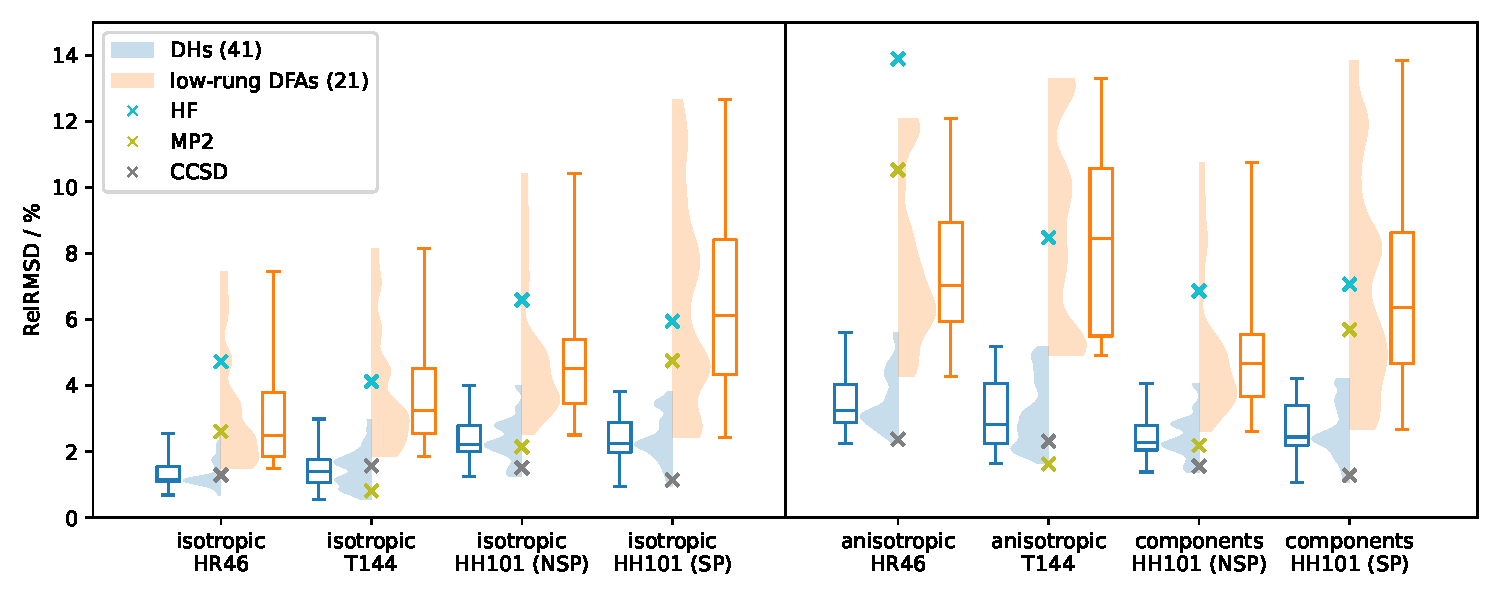
\includegraphics[width=0.8\textwidth]{assets/benchmark-compare-dh-low.pdf}
    \caption{诸双杂化泛函 (DH) 与诸低阶泛函 (low-rung DFA) 泛函极化率数据集相对方均根误差 (RelRMSD) 测评表现图。小提琴图的数据密度建模方式是 Gaussian 核,参数 \texttt{bw\_method} 设为 0.2。箱型图展示了密度泛函测评误差的 1/4 位次、中位次、3/4 位次误差。图例中括号数字表示其对应分类被测评的泛函数量。}
    \label{fig.6.benchmark-compare-dh-low}
\end{figure}

首先对所有泛函总体表现作简要的测评。图 \ref{fig.6.benchmark-compare-dh-low} 展示了双杂化泛函与低阶泛函的总体误差表现、以及这两者之间的对比情况:
\begin{itemize}[nosep]
    \item 对于所有泛函,HR46 与 T144 数据集的异性极化率 $\gamma$ 误差都大于同性极化率 $\alpha$ 误差。对于双杂化泛函,HR46 与 T144 数据集的异性极化率 $\gamma$ 误差平均比同性极化率 $\alpha$ 误差分别大 2.14\% 与 1.69\%;对于低阶泛函,误差分别增大了 4.43\% 与 4.80\%。这也意味着同性极化率 $\alpha$ 与异性极化率 $\gamma$ 的误差表现有必要分开讨论。
    \item 对于所有泛函,HH101 数据集的分量 $\alpha_{xx}, \alpha_{yy}, \alpha_{zz}$ 大于同性极化率 $\alpha$ 误差;但增幅并不大,且泛函误差分布情况也非常相近。对于双杂化泛函,HH101 数据集的自旋非极化 (NSP) 与极化 (SP) 子集的分量 $\alpha_{xx}, \alpha_{yy}, \alpha_{zz}$ 误差平均比同性极化率 $\alpha$ 误差分别大 0.06\% 与 0.28\%;对于低阶泛函,误差分别增大了 0.17\% 与 0.45\%。因此,尽管分量 $\alpha_{xx}, \alpha_{yy}, \alpha_{zz}$ 作为与同性极化率 $\alpha$ 不同的测评标准,其测评结果可以一定程度地反映极化率在各分量上的表现;但其测评结果与同性极化率 $\alpha$ 非常相近。
    \item 双杂化泛函在所有数据集上的表现明显优于低阶泛函;即使是如 MPW1K、SCAN0 等低阶泛函中表现最好的泛函,其误差也仍然高于所测评的双杂化泛函误差的中位数。
    \item 双杂化泛函中表现最好的泛函,可以在 HR46、HH101 数据集上与 CCSD 有相近的良好误差表现,在 T144 数据集上与 MP2 有相近的良好误差表现。
\end{itemize}

在极化率计算问题上,双杂化泛函的计算误差显著小于低阶泛函;而相比于高精度波函数方法,双杂化泛函可能同时大幅降低计算量、但同时有更精准的计算结果。对于双杂化泛函优异的极化率表现,我们对此作如下理解。

回顾第 \alertref{sec.3.title} 章,xDH 泛函的静态电性质的计算可以归结为分子总能量 $E^\textsf{xDH}$ 对外场 $\symbfcal{E}$ 的梯度计算;偶极矩 $t \in \{ x, y, z \}$ 分量的计算可以化归为问题
\begin{equation*}
    \mu_t^\textsf{xDH} = \partial_{\mathcal{E}_t} E^\textsf{xDH} = D_{pq}^\textsf{xDH} F_{pq}^{\mathcal{E}_t} + \partial_{\mathcal{E}_t} E^\textsf{non-elec}
\end{equation*}
该式的 $\partial_{\mathcal{E}_t} E^\textsf{non-elec}$ 一般情况下是原子核受外电场影响下的能量变化,与电子结构方法无关。如果将分子轨道下的密度矩阵作基变换到原子轨道下:
\begin{equation*}
    D_{\mu \nu}^\textsf{xDH} = D_{pq}^\textsf{xDH} C_{\mu p} C_{\nu q}
\end{equation*}
则偶极矩的计算问题可以继续化归为
\begin{equation}
    \mu_t^\textsf{xDH} = D_{\mu \nu}^\textsf{xDH} F_{\mu \nu}^{\mathcal{E}_t} + \partial_{\mathcal{E}_t} E^\textsf{non-elec}
\end{equation}
其中 $F_{\mu \nu}^{\mathcal{E}_t}$ 作为电性质 Skeleton 导数,也仅与分子结构有关,而与电子结构无关。因而,可以左右计算电子结构在偶极矩计算问题上计算表现的唯一变量,是该方法的弛豫密度矩阵 $D_{\mu \nu}^\textsf{xDH}$。对于 bDH 型泛函、以及低阶泛函,它们可以看做是 xDH 泛函的退化形式,即上式对 bDH 与低阶泛函也同样成立。作为密度矩阵的导出量,第四章的测评已经表明双杂化泛函的密度 $\rho^\textsf{xDH} (\bm{r}) = D_{\mu \nu}^\textsf{xDH} \phi_\mu (\bm{r}) \phi_\nu (\bm{r})$ 及其关于空间坐标的梯度,有良好的表现;而在 Hait 与 Head-Gordon 的工作\cite{Hait-Head-Gordon.JCTC.2018}中,双杂化泛函也有良好的偶极矩测评结果。

极化率分量 $t, s \in \{ x, y, z \}$ 则是偶极矩在偶极外场下的梯度:
\begin{equation*}
    \alpha_{ts} = - \partial_{\mathcal{E}_s} \partial_{\mathcal{E}_t} E^\textsf{xDH} = - \big( \partial_{\mathcal{E}_s} D_{\mu \nu}^\textsf{xDH} \big) F_{\mu \nu}^{\mathcal{E}_t}
\end{equation*}
因此,与偶极矩类似地,可以左右计算电子结构在极化率计算问题上计算表现的唯一变量,是该方法弛豫密度矩阵在偶极电场下的微扰响应 $\partial_{\mathcal{E}_s} D_{\mu \nu}^\textsf{xDH}$。因此,我们认为双杂化泛函在极化率计算问题上有良好的表现,其根本的原因是对 $\partial_{\mathcal{E}_s} D_{\mu \nu}^\textsf{xDH}$ 有成功的描述。

\subsection{双杂化泛函误差测评与讨论}

\begin{figure}[hp]
    \centering
    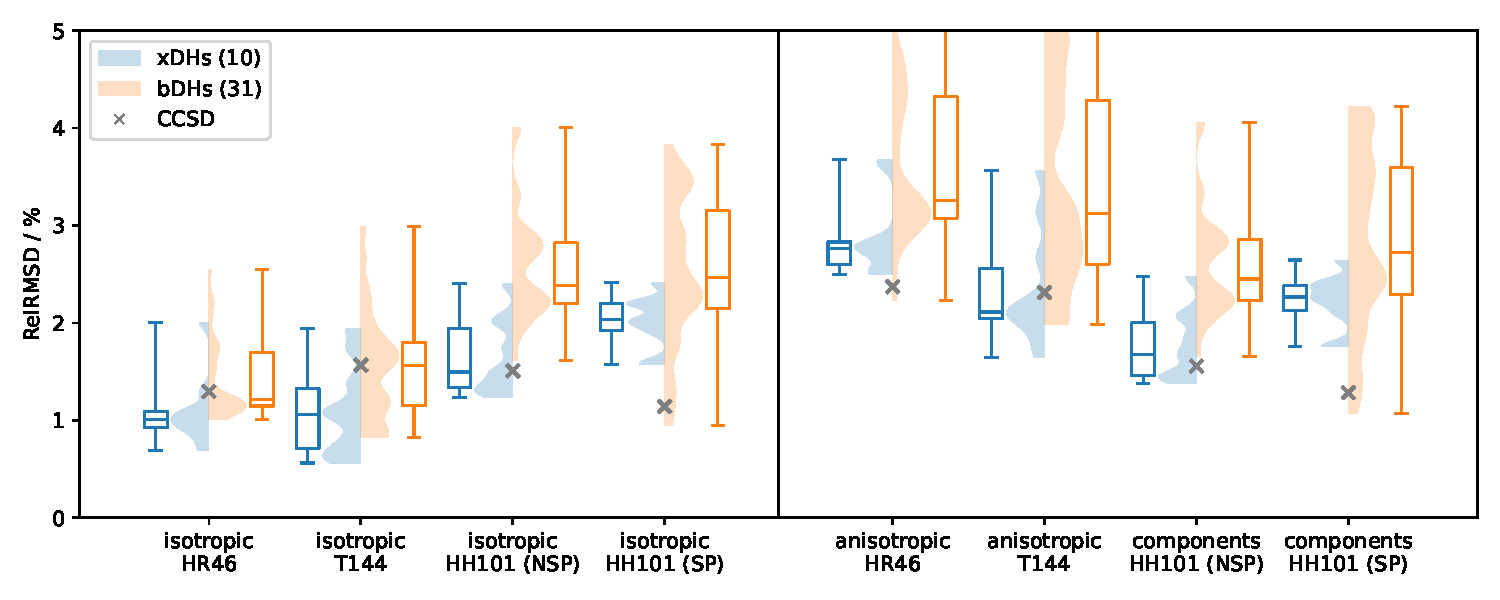
\includegraphics[width=0.8\textwidth]{assets/benchmark-compare-xdh-bdh.pdf}
    \caption{诸 XYG3 型双杂化泛函 (xDH) 与诸 B2PLYP 型双杂化泛函 (bDH) 泛函极化率数据集相对方均根误差 (RelRMSD) 测评表现图。图例参考图 \ref{fig.6.benchmark-compare-dh-low}。}
    \label{fig.6.benchmark-compare-xdh-bdh}
\end{figure}

随后对不同类型的双杂化的误差作更细致的讨论。图 \ref{fig.6.benchmark-compare-xdh-bdh} 展示了 xDH 型泛函与 bDH 型泛函误差的比较示意图。可以看到,对于 HR46 同性极化率 $\alpha$、T144 数据集以及 HH101 自旋非极化分子子集,比之于 bDH 型泛函,xDH 型泛函的总体表现与最低误差都更好。作为特例,在 HR46 异性极化率 $\gamma$ 数据集上,DSD-PBEPBE-D3BJ 的 RelRMSD 误差是 2.23\%,比 xDH 型泛函中误差最低的 revXYG3 (2.49\%) 更低一些;但除此泛函以及 DSD-PBEP86-D3BJ (2.56\%) 之外,其余的 bDH 型泛函误差都比除 XYG-OS5 (3.68\%) 外的所有经测评的 xDH 泛函误差更大。因此,我们认为,诸多 xDH 型泛函在 HR46 与 T144 等中等分子的、以自旋非极化体系为主的数据集上,不论是同性极化率 $\alpha$ 还是异性极化率 $\gamma$,都有较为稳定且优异的误差表现。

但 HH101 自旋极化分子子集上,xDH 泛函尽管在平均表现上比 bDH 型泛函更好,但更多的 bDH 型泛函在该数据集上展现出优势。为简化讨论,我们仅考察 HH101 自旋极化子集的同性极化率 $\alpha$ 测评结果。在该数据集上,表现较好的 xDH 型泛函是 XYG7 (1.58\%)、XYGJ-OS (1.59\%)、XYG6 (1.91\%);而 bDH 型泛函中,ωPBEPP86 (0.95\%)、ωB88PP86 (1.13\%)、DSD-PBEP86-D3BJ (1.32\%)、DSD-PBEPBE-D3BJ (1.41\%) 的表现相当出色。除此之外,ωB2GP-PLYP (1.83\%) 也有较好的误差表现。我们注意到,ωPBEPP86、ωB88PP86、ωB2GP-PLYP 等泛函在交换部分包含长短程矫正。

\begin{figure}[hp]
    \centering
    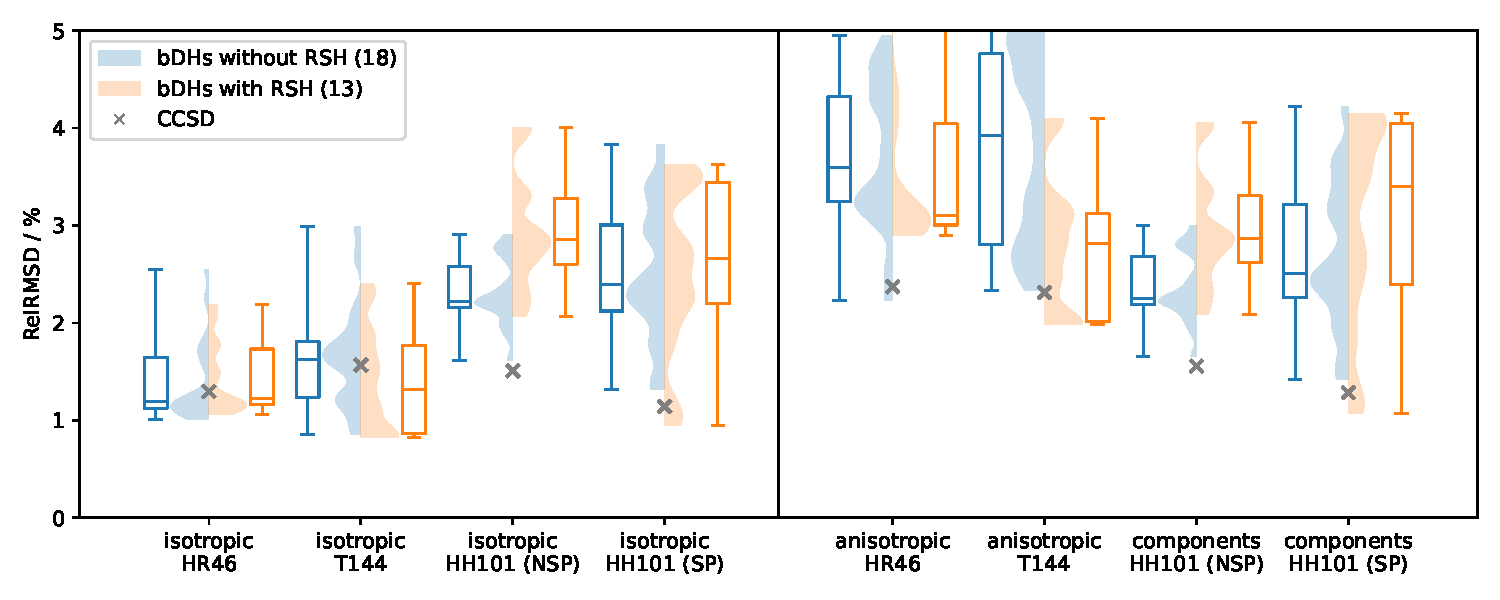
\includegraphics[width=0.8\textwidth]{assets/benchmark-compare-dh-rsh.pdf}
    \caption{诸 bDH 型双杂化泛函依交换部分是否为 RSH 型泛函而分类的极化率数据集相对方均根误差 (RelRMSD) 测评表现图。图例参考图 \ref{fig.6.benchmark-compare-dh-low}。}
    \label{fig.6.benchmark-compare-dh-rsh}
\end{figure}

由于本工作不涉及交换部分 RSH 型的 xDH 型泛函,因此这里在测评交换部分 RSH 对极化率误差表现时,我们仅考察 bDH 型双杂化泛函。误差表现展示于图 \ref{fig.6.benchmark-compare-dh-rsh}。可以发现,RSH 项的引入确实提升了部分泛函在 HH101 自旋非极化数据集的测评表现,但交换部分 RSH 型泛函总体表现并非总是比非 RSH 型泛函更具有优势。我们还发现,交换部分 RSH 型泛函的测评表现与泛函的构成风格有较大关系:
\begin{itemize}[nosep]
    \item RSX-QIDH、SOS-RSX-PBE-QIDH 等泛函是非参数优化的泛函;它们的表现相对一般;
    \item ωPBEPP86、ωB88PP86、ωB2GP-PLYP、ωB2PLYP 等泛函是专门针对激发态计算所优化;这些泛函在 HH101 数据集上有较好的表现;
    \item RS-B88-LYP、RS-PBE-PBE、RS-PBE-P86、RS-PW91-PW91 等泛函也专门针对激发态作优化,但在泛函形式上还包含相关部分 RSH 的贡献;这些泛函在 T144 数据集上有较好的表现,但在 HH101 自旋极化子集上表现较差。
\end{itemize}
因此,尽管对双杂化泛函引入 RSH 项,确实可以提升部分静态极化率数据集的评测表现;但 RSH 项并非唯一的影响因素、也并非能保证在所有静态极化率计算问题上有所提升。

\section{xDH@B3LYP 模型静态极化率参数优化}
\label{sec.6.pol-xdh-optimize}

\begin{sidewaystable}
\centering
\caption{以 WTRE 误差量标优化的 xDH@B3LYP 模型静态极化率参数,及各静态极化率数据集误差结果${}^3$。}
\label{tab.6.xdh-b3lyp-polar-opt}
\widetabular{
    \begin{tabular}{lld{2.7}d{2.7}d{2.7}d{2.7}d{2.7}d{2.7}d{2.7}d{2.7}}
    \toprule
    & & \multicolumn{1}{c}{B3LYP} & \multicolumn{1}{c}{XYG3} & \multicolumn{1}{c}{XYG5} & \multicolumn{1}{c}{XYG6} & \multicolumn{1}{c}{XYG7} & \multicolumn{1}{c}{XYG-OS3} & \multicolumn{1}{c}{XYGJ-OS} & \multicolumn{1}{c}{XYG-OS5} \\
    \midrule
    泛函参数\tnote{b}
    & $a_1$ ($E_\mathrm{x}^\text{exact}$) & 0.330646   & 0.887385   & 0.843480   & 0.707769   & 0.714877  & 0.794151 & 0.667163   & 0.681864   \\
    & $a_2$ ($E_\mathrm{x}^\text{S}$) & [0.113675] & [0.297922] & [0.231657] & [0.520989] & 0.523649  & [0.205849] & [0.332837] & [0.338714] \\
    & $a_3$ ($E_\mathrm{x}^\text{B88}$) & 0.555679   & -0.185307  & -0.075137  & -0.228758  & -0.259884 & [0.{\color{white}000000}]     & [0.{\color{white}000000}] & -0.020578  \\
    & $a_4$ ($E_\mathrm{c}^\text{VWN3}$) & [0.741727] & [0.{\color{white}000000}] & [0.{\color{white}000000}] & 0.995154   & 1.271473  & [0.{\color{white}000000}] & 0.883246   & 1.120226   \\
    & $a_5$ ($E_\mathrm{c}^\text{LYP}$) & 0.258273   & [0.659253] & 0.615211   & -0.667102  & -0.811699 & 0.673447 & -0.500754  & -0.614148  \\
    & $a_6$ ($E_\mathrm{c}^\text{OS-PT}$) & [0.{\color{white}000000}] & 0.340747   & 0.408184   & 0.365681   & 0.371477  & 0.419592 & 0.353082   & 0.359351   \\
    & $a_7$ ($E_\mathrm{c}^\text{SS-PT}$) & [0.{\color{white}000000}] & [0.340747] & 0.115199   & 0.049551   & 0.038238  & [0.{\color{white}000000}] & [0.{\color{white}000000}] & [0.{\color{white}000000}] \\
    \midrule
    同性极化率\tnote{c}
    & HR46        & 1.365      & 0.926      & 0.739      & 0.560      &0.553     & 0.720    & 0.637      & 0.661      \\
    & T144        & 2.102      & 1.004      & 0.729      & 0.794      &0.784     & 0.668    & 0.875      & 0.867      \\
    & HH101 (NSP) & 2.307      & 1.341      & 0.815      & 0.879      &0.971     & 0.913    & 0.800      & 0.853      \\
    & HH101 (SP)  & 3.577      & 2.158      & 2.035      & 1.288      & 1.106     & 2.118    & 1.281      & 1.123      \\ \midrule
    异性极化率\tnote{c}
    & HR46        & 5.201      & 2.185      & 2.238      & 2.290      &2.322     & 2.565    & 2.537      & 2.585      \\
    & T144        & 6.007      & 2.343      & 1.826      & 2.252      & 2.205     & 1.853    & 2.431      & 2.367      \\ \midrule
    极化率分量\tnote{c}
    & HH101 (NSP) & 2.398      & 1.431      & 0.998      & 1.020      &1.131     & 1.118    & 0.942      & 1.003      \\
    & HH101 (SP)  & 3.725      & 2.395      & 2.237      & 1.418      & 1.240     & 2.306    & 1.410      & 1.259      \\ \midrule
    WTRE\tnote{d}
                &             & 0.884      & 0.471      & 0.388      & 0.347      & 0.342     & 0.405    & 0.360      & 0.356      \\ \bottomrule
    \end{tabular}
}{
    \item[a] 该表格的泛函名称 (如 B3LYP、XYG7 等) 并不指代业已发表的泛函,而是指代其对应的参数模型。B3LYP 参数模型参考 Stephens 等人工作\cite{Stephens-Frisch.JPC.1994},XYG-OS3 为本工作的参数模型,其余参数模型参考张颖与徐昕的工作\cite{Zhang-Xu.JPCL.2021}。
    \item[b] 该参数表的定义参考张颖与徐昕的工作\cite{Zhang-Xu.JPCL.2021},或参考表 \alertref{tab.2.coeff-xyg6-1-weighted-error}。
    \item[c] 测评误差以 RelRMSD (\%) 表示。
    \item[d] 加权相对误差的定义参考式 (\ref{eq.6.wtre}) 附近的讨论。
}
\end{sidewaystable}

这一节将基于 xDH@B3LYP 参数化模型\cite{Zhang-Xu.JPCL.2021},仅针对极化率测评表现进行参数优化。需要指出,本节所涉及的泛函名称 (如 XYG7、B3LYP 等) 可能指代其对应的参数化模型,而并非指代业已发表的泛函本身。本节的参数优化仅适用于静态极化率测评与分析;既不额外引入基于能量或结构等测评结果、也未引入对泛函公式形式的物理限制的前提下,我们认为这里的泛函参数优化过程并非是对普适泛函的一种逼近策略。

表 \ref{tab.6.xdh-b3lyp-polar-opt} 展示了针对极化率的加权相对误差量标 WTRE,xDH@B3LYP 模型下的参数优化结果与测评误差。可以看到,
\begin{itemize}[nosep]
    \item 原始的 B3LYP 泛函的 WTRE 误差为 1.647;而对 B3LYP 三参数模型作优化后,其 WTRE 误差降低到 0.884,与本工作所被测评的最好的低阶泛函 MPW1K 的 WTRE 误差 0.877 较为接近。这一方面表明,对于类似于 B3LYP 等的低阶泛函,其极化率表现可以通过参数重新优化得到大幅提升;但另一方面,在没有引入二阶微扰贡献的前提下,即使放开 B3LYP 的三参数优化,也难以达到普通双杂化泛函的极化率计算误差表现。这加强了先前泛函测评得到的结论,即双杂化泛函的表现明显优于低阶泛函。
    \item 除 XYG3 之外,其余 xDH@B3LYP 泛函的参数化模型都可以优化得到 0.41 以下的 WTRE (在表 \ref{tab.6.full-benchmark} 所测评的泛函中,表现最好的是 XYGJ-OS,其 WTRE 为 0.418)。这意味着放开部分或所有 xDH@B3LYP 模型参数确实可以提升静态极化率测评表现。但同时需要指出,当放开所有参数时,XYG7 参数化模型的 WTRE 误差仍然有 0.342;该误差并未比原始的 XYGJ-OS 泛函误差 0.418 小许多。因此,对 xDH@B3LYP 模型参数放开优化确实有所提升,但提升较为有限。
    \item 对于同时放开 VWN3 型相关能参数 $a_4$ 与 LYP 型相关能参数 $a_5$ 的情形 (XYG6, XYG7, XYGJ-OS, XYG-OS5 四种模型),参数 $a_5$ 的数值会产生相当严重的负值、同时参数 $a_4$ 有较大的数值;这些参数化模型给出的 WTRE 误差也相对较小 (在 0.34--0.36 之间)。但考虑到 xDH@B3LYP 参数化模型在对诸如 GMTKN55 等反应能误差量标下,参数优化很少遇到这种严重负值的情形;且同时放开 $a_4$ 与 $a_5$ 参数优化的极化率测评 WTRE 误差表现并不显著地比冻结其中一者优化的情形有优势 (XYG5 模型或 XYG-OS3 模型的误差在 0.38--0.41 之间);因此我们担忧,过度放开参数优化限制、且仅针对极化率问题作参数优化,尽管在 WTRE 量标上有微少的提升,但却会导出偏离物理图像或直觉的泛函。
    \item 在放开同自旋二阶微扰贡献项 $E_\mathrm{c}^\text{SS-PT}$ 的 $a_7$ 参数模型中 (XYG5, XYG6, XYG7 三种模型),所有优化得到的 $a_7$ 参数接近零值 (均小于 0.12)。而若将 $a_7$ 参数置零,如 XYG-OS5 模型之于 XYG6 模型,误差不会显著地提升。而对比 XYG3 模型与 XYG-OS3 模型,可以发现同样为三参数模型,XYG-OS3 模型静默 $a_7$ 参数的 WTRE 误差 0.41 明显小于 XYG3 模型的 0.47。因此,限制 $E_\mathrm{c}^\text{SS-PT}$ 的贡献、或合理地分离二阶微扰的两种自旋贡献 $E_\mathrm{c}^\text{OS-PT}$ 与 $E_\mathrm{c}^\text{SS-PT}$,可以有效地提升极化率测评表现。
\end{itemize}

\section{本章小结}

基于对双杂化泛函的极化率测评的目的,本章展开了一系列分析、验证与测评工作。

为确认一种高效且具有足够精度的计算基组,我们以 B2PLYP 泛函作为双杂化泛函的典型,作细致的基组收敛性分析;并最终估计 aug-pc-3 基组作为计算代价较小的基组,其同性极化率 $\alpha$ 或异性极化率 $\gamma$ 的 BSIE 误差在 0.5\% 误差范围内。我们认为,以该基组作为双杂化或低阶泛函的静态极化率测评是合适的。

我们对诸多双杂化与低阶泛函,对 HR46、T144、HH101 三个数据集的同性极化率 $\alpha$,HR46 与 T144 两个数据集的异性极化率 $\gamma$,以及 HH101 数据集极化率分量 $\alpha_{xx}, \alpha_{yy}, \alpha_{zz}$ 作系统的测评。这部分测评表明,双杂化泛函的极化率误差显著地小于低阶泛函的误差;且表现最优异的双杂化泛函,在以 CCSD(T) 为基准的前提下,其误差可以媲美波函数方法 MP2、或计算开销上更为昂贵 CCSD 或甚至更小。双杂化泛函适合用于以 HR46、T144、HH101 为代表的一系列中小分子的静态极化率计算;而在其中,以 XYGJ-OS、XYG6、xDH-PBE0 为代表的 xDH 型泛函,与 DSD-PBEPBE-D3BJ 为代表的 bDH 型泛函,在各极化率数据集上有相当低的误差表现,是适合用于静态极化率计算的双杂化泛函。

本工作还对各种 xDH@B3LYP 模型下的泛函作参数优化的尝试。我们发现,异自旋二阶微扰贡献项 $E_\mathrm{c}^\text{OS-PT}$ 对于静态极化率的描述有重要的作用;即在合理的泛函构造下,双杂化泛函确实比专门针对极化率作参数优化的低阶泛函,有更低的误差。同时,当同自旋二阶微扰贡献项 $E_\mathrm{c}^\text{SS-PT}$ 贡献相比于 $E_\mathrm{c}^\text{OS-PT}$ 较少甚至于零贡献时,双杂化泛函的极化率误差通常较小。专门针对静态极化率而优化的 xDH@B3LYP 模型泛函确实有更好的极化率表现,但也容易产生非物理或不符合直觉的泛函参数,测评误差的提升也比较有限;考虑到密度泛函的泛用性,我们认为使用以 XYGJ-OS、XYG6、xDH-PBE0、DSD-PBEPBE-D3BJ 为代表的基于能量误差量标优化的泛函,也可以很好地描述静态极化率。

\newpage

\section{附录}

\subsection{对 HH132 数据集自旋极化体系准确性的讨论}
\label{sec.6.supp-HH132-remove}

在我们的测评与验证过程中,我们发现对于 HH132 数据集\cite{Hait-Head-Gordon.PCCP.2018}的 57 个自旋极化体系,其许多体系的计算本身存在挑战、我们的计算结果和 HH132 数据集的参考值与测评值也存在差异。在正文中,我们仅对其中部分自旋极化体系作测评与统计;在这里,我们将详细地讨论复现 HH132 数据集过程中遇到的困难,并指出测评过程中剔除部分自旋极化体系的具体原因。

\subsubsection{对称性破缺}

在 HH132 的 57 个自旋极化分子中,13 个分子的电子态存在对称性破缺效应;因此解析极化率的计算与数值极化率有所不同。相关的数据列于表 \ref{tab.6.supp.symm-broken}。这些分子中,
\begin{itemize}[nosep]
    \item 以平均场的分子轨道讨论,\ce{BN}, \ce{NO}, \ce{OCl}, \ce{OF}, \ce{OH}, \ce{SCl}, \ce{SF}, \ce{SH}, \ce{PS}, \ce{NCO} 这 10 个 $C_{\infty v}$ 对称性自由基由于存在单电子占据的 $\Pi$ 不可约表示下的轨道,因此电子云在垂直于主轴的面上并不是均匀分布的 (即当主轴为 $z$ 轴时,电子云的分布在 $x$ 方向与 $y$ 方向并不相同)。依数值差分方法给出极化率,若电子占据轨道没有特定不可约表示的限制,那么在施加垂直于 $z$ 轴的外偶极电场时,电子云总是会旋转到能量更低的状态,而不是反映无外电场时的分布,因此会给出 $\alpha_{xx} = \alpha_{yy}$ 的结论;这也与 HH132 数据集的结果表现一致。但解析梯度给出的极化率可以反映无外电场时电子云的分布,即 $\alpha_{xx}$ 未必等于 $\alpha_{yy}$。我们认为,解析梯度的极化率是理论上严格的极化率计算方式;因此,我们决定在采用 HH132 数据集参考值时,排除这 10 个存在单电子占据的  $\Pi$ 不可约表示的 $C_{\infty v}$ 对称性自由基体系。
    \item 与上述原因类似地,我们排除 $C_{3v}$ 对称性下存在单电子占据 $E$ 不可约表示轨道的自由基 \ce{CH3O}。除此之外,该体系的解析极化率本身计算也容易产生数值问题。
    \item \ce{Be} 原子与 \ce{Li2} 分子则是在自洽场计算中,存在对称性更低、但能量上更稳定的态 (分别是 $C_{\infty v}$ 与 $C_s$);从而上述原因也会应用到这两个体系,导致不限制电子占据轨道不可约表示的数值极化率计算、与解析极化率在结果上存在差异。
\end{itemize}

\begin{table}[!ht]
\centering
\caption{HH132 数据集中存在对称性破缺问题的分子及极化率结果${}^a$。}
\label{tab.6.supp.symm-broken}
\widetabular{
    \begin{tabular}{lld{4.4}d{2.3}d{2.3}d{2.3}d{2.3}d{2.3}}
    \toprule
    & & \multicolumn{3}{c}{解析极化率 / $\text{\AA}{}^{3}$\tnote{b}} & \multicolumn{3}{c}{HH132 原始数据 / $\text{\AA}{}^{3}$\tnote{c}} \\
    \cmidrule(lr){3-5} \cmidrule(lr){6-8}
    点群 & 体系 & \multicolumn{1}{c}{$\alpha_{xx}$} & \multicolumn{1}{c}{$\alpha_{yy}$} & \multicolumn{1}{c}{$\alpha_{zz}$} & \multicolumn{1}{c}{$\alpha_{xx}$} & \multicolumn{1}{c}{$\alpha_{yy}$} & \multicolumn{1}{c}{$\alpha_{zz}$} \\
    \midrule
    $SO(3)$                          & \ce{Be  } & 7.019      & 7.019    & 7.667   & 7.074      & 7.074     & 7.074     \\
    \midrule
    $D_{\infty h}$                   & \ce{Li2 } & 26.837     & 22.980   & 39.702  & 24.529     & 24.529    & 24.529    \\
    \midrule
    $C_{\infty v}$ & \ce{BN  } & 3.427      & 2.521    & 2.156   & 3.446      & 3.446     & 2.161     \\
    & \ce{NO  } & 1.444      & 1.240    & 0.434   & 1.445      & 1.445     & 0.557     \\
    & \ce{OCl } & 2.475      & 2.390    & 4.289   & 2.391      & 2.391     & 4.296     \\
    & \ce{OF  } & 1.057      & 1.081    & 1.814   & 1.057      & 1.057     & 1.816     \\
    & \ce{OH  } & 1.071      & 0.879    & 1.244   & 1.072      & 1.072     & 1.245     \\
    & \ce{SCl } & 4.065      & 4.387    & 7.137   & 4.393      & 4.393     & 7.147     \\
    & \ce{SF  } & 3.170      & 2.786    & 3.592   & 3.178      & 3.178     & 3.594     \\
    & \ce{SH  } & 2.875      & 3.449    & 3.446   & 3.458      & 3.458     & 3.450     \\
    & \ce{PS  } & 5.687      & 5.152    & 12.050  & 5.159      & 5.159     & 11.985    \\
    & \ce{NCO } & 2.264      & 2.232    & 4.005   & 2.233      & 2.233     & 4.028     \\
    \midrule
    $C_{3v}$                         & \ce{CH3O} & -318.402\tnote{d} & 2.644    & 3.326   & 4.080      & 2.762     & 3.330     \\
    \bottomrule
    \end{tabular}
}{
    \item[a] 表中所列的分子均为极化率张量 $\bm{\alpha}$ 不满足分子点群对称性的情形。列表中所展示的点群是分子构型对应的点群。计算模型是 MP2/aCVTZ。
    \item[b] 解析极化率由 \textsc{Gaussian 16} (rev B01)\cite{Gaussian16} 计算。该计算开启默认的对称性 (\ce{CH3O} 分子构型接近 $C_{3v}$,但程序中使用 $C_s$ 计算)。
    \item[c] 数据来自于 HH132 数据集原文\cite{Hait-Head-Gordon.PCCP.2018}。
    \item[d] \ce{CH3O} 自由基的解析 $\alpha_{xx}$ 分量数值确实存在异常;这在 \textsc{dh} 程序给出的结果中尽管具体数值不同,但也存在相当严重的误差。
}
\end{table}

\subsubsection{MP2 极化率复现问题}

通过解析梯度计算复现 HH132 数据集的 MP2/aCVTZ 数值极化率数据时,我们认为部分体系误差较大。其中,由 \textsc{Gaussian 16} 解析计算的极化率与 HH132 原始数据集中存在大于 2\% 差异的体系有 5 个,如表 \ref{tab.6.supp.mp2-hait-g16} 所示。这些分子中,\ce{CH2NH}, \ce{NOCl}, \ce{NaLi} 使用不同的程序下给出的解析极化率也有一定程度上的不同,如表 \ref{tab.6.supp.mp2-dh-g16} 所示;这表明这些分子的电子云在 MP2/aCVTZ 模型下并不稳定,其极化率容易受外场或数值精度的影响而产生大幅改变。由于 HH132 数据集中的 MP2 极化率结果是 CCSD(T) 参考值结果的中间输出,因此我们认为,若 MP2 的计算偏差较大、那么作为参考值的 CCSD(T) 也很可能存在无法忽视的偏差;从而这些分子体系不适合使用 HH132 的参考值对诸泛函作测评。

\begin{table}[!ht]
\centering
\caption{HH132 数据集解析与数值极化率相对误差超过 2\% 的体系、及其极化率数值与误差${}^a$。}
\label{tab.6.supp.mp2-hait-g16}
\widetabular{
    \begin{tabular}{ld{3.3}d{3.3}d{3.3}d{4.4}d{4.4}d{4.4}}
    \toprule
    & \multicolumn{3}{c}{解析极化率 / $\text{\AA}{}^{3}$\tnote{b}} & \multicolumn{3}{c}{相对误差 / \%\tnote{c}} \\
    \cmidrule(lr){2-4} \cmidrule(lr){5-7}
    体系 & \multicolumn{1}{c}{$\alpha_{xx}$} & \multicolumn{1}{c}{$\alpha_{yy}$} & \multicolumn{1}{c}{$\alpha_{zz}$} & \multicolumn{1}{c}{$\alpha_{xx}$} & \multicolumn{1}{c}{$\alpha_{yy}$} & \multicolumn{1}{c}{$\alpha_{zz}$} \\
    \midrule
    \ce{CH2NH} & 3.299    & 2.713    & 6.678    & 0.129       & 0.191      & -115.065    \\
    \ce{HOF  } & 1.443    & 1.254    & 4.023    & 0.028       & 0.061      & -40.274     \\
    \ce{NOCl } & 5.814    & 6.487    & 3.452    & -67.820     & -8.420     & 0.075       \\
    \ce{Na2  } & 30.066   & 30.066   & 26.148   & 0.069       & 0.069      & 2.452       \\
    \ce{NaLi } & 26.443   & 26.443   & -11.852  & 0.100       & 0.100      & -18.332     \\
    \bottomrule
    \end{tabular}
}{
    \item[a] 该表格的分析中,去除了表 \ref{tab.6.supp.symm-broken} 所涉及的 13 个分子。计算模型是 MP2/aCVTZ。
    \item[b] 解析极化率由 \textsc{Gaussian 16} (rev B01)\cite{Gaussian16} 计算。
    \item[c] 相对误差是指 HH132 数值极化率相对于 \textsc{Gaussian 16} 计算得到的解析极化率的比值误差。
}
\end{table}

\begin{table}[!ht]
\centering
\caption{HH132 数据集不同程序 (\textsc{dh} 与 \textsc{Gaussian 16}) 解析极化率相对误差超过 0.5\% 的体系、及其极化率数值与误差${}^a$。}
\label{tab.6.supp.mp2-dh-g16}
\widetabular{
    \begin{tabular}{ld{3.3}d{3.3}d{3.3}d{3.3}d{3.3}d{3.3}}
    \toprule
    & \multicolumn{3}{c}{解析极化率 / $\text{\AA}{}^{3}$\tnote{b}} & \multicolumn{3}{c}{相对误差 / \%\tnote{c}} \\
    \cmidrule(lr){2-4} \cmidrule(lr){5-7}
    体系 & \multicolumn{1}{c}{$\alpha_{xx}$} & \multicolumn{1}{c}{$\alpha_{yy}$} & \multicolumn{1}{c}{$\alpha_{zz}$} & \multicolumn{1}{c}{$\alpha_{xx}$} & \multicolumn{1}{c}{$\alpha_{yy}$} & \multicolumn{1}{c}{$\alpha_{zz}$} \\
    \midrule
    \ce{CH2NH} & 3.299  & 2.713  & 6.678   & 0.160 & 0.073  & 22.152 \\
    \ce{NOCl } & 5.814  & 6.487  & 3.452   & 4.268 & 4.564  &  0.017 \\
    \ce{NaLi } & 26.443 & 26.443 & -11.852 & 0.225 & 0.225  & -9.846 \\
    \bottomrule
    \end{tabular}
}{
    \item[a] 该表格的分析中,去除了表 \ref{tab.6.supp.symm-broken} 所涉及的 13 个分子。计算模型是 MP2/aCVTZ。\textsc{dh} 程序计算结果使用 ETB 辅助基组。
    \item[b] 解析极化率由 \textsc{Gaussian 16} (rev B01)\cite{Gaussian16} 计算。
    \item[c] 相对误差是 \textsc{dh} 计算得到的解析极化率、相对于 \textsc{Gaussian 16} 计算得到的解析极化率的比值误差。
}
\end{table}

\subsubsection{其他双杂化泛函复现或数值问题}

\begin{table}[!htp]
\centering
\caption{HH132 数据集部分双杂化泛函 aCVTZ 数据与解析极化率相对误差超过 2\% 的体系、及其极化率数值与误差${}^a$。}
\label{tab.6.supp.double-hybrid-hh132-g16}
\widetabular{
    \begin{tabular}{llld{1.3}d{1.3}d{1.3}d{3.3}d{3.3}d{3.3}}
    \toprule
    & & & \multicolumn{3}{c}{解析极化率 / $\text{\AA}{}^{3}$\tnote{b}} & \multicolumn{3}{c}{相对误差 / \%\tnote{c}} \\
    \cmidrule(lr){4-6} \cmidrule(lr){7-9}
    泛函 & 体系 & 自旋极化 & \multicolumn{1}{c}{$\alpha_{xx}$} & \multicolumn{1}{c}{$\alpha_{yy}$} & \multicolumn{1}{c}{$\alpha_{zz}$} & \multicolumn{1}{c}{$\alpha_{xx}$} & \multicolumn{1}{c}{$\alpha_{yy}$} & \multicolumn{1}{c}{$\alpha_{zz}$} \\
    \midrule
    B2PLYP & \ce{C2H  } & SP  & 3.543 & 3.543 & 4.020  & 8.564   & 8.564   & -0.127  \\
    53\% $E_\mathrm{x}^\mathrm{exact}$ & \ce{CN   } & SP  & 3.192 & 3.192 & 4.518  & -18.839 & -18.839 & -2.985  \\
    & \ce{HNS  } & SP  & 5.796 & 3.959 & 3.031  & -1.502  & 3.246   & 10.542  \\
    & \ce{NaCl } & NSP & 4.334 & 4.334 & 5.471  & 0.698   & 0.698   & 2.058   \\
    & \ce{O3   } & SP  & 1.713 & 4.580 & 2.124  & 0.000   & -4.345  & -1.471  \\
    \midrule
    B2GPPLYP      & \ce{C2H  } & SP  & 3.395 & 3.395 & 4.009  & 7.009   & 7.009   & -0.751  \\
    65\% $E_\mathrm{x}^\mathrm{exact}$ & \ce{CN   } & SP  & 3.304 & 3.304 & 4.243  & -18.696 & -18.696 & -1.834  \\
    & \ce{HNO  } & SP  & 1.490 & 2.289 & 2.719  & 5.253   & 0.786   & 1.883   \\
    & \ce{HNS  } & SP  & 6.974 & 3.971 & 4.786  & -18.989 & 1.673   & -30.387 \\
    & \ce{NP   } & SP  & 3.357 & 3.357 & 6.635  & 6.480   & 6.480   & -18.120 \\
    & \ce{O2   } & SP  & 1.174 & 1.174 & 2.193  & 0.372   & 0.372   & -3.047  \\
    & \ce{O3   } & SP  & 1.696 & 4.518 & 2.095  & 0.226   & -4.981  & -1.451  \\
    \midrule
    DSD-PBEPBE-D3 & \ce{BO   } & SP  & 2.308 & 2.308 & 2.790  & 0.141   & 0.141   & 3.479   \\
    69\% $E_\mathrm{x}^\mathrm{exact}$ & \ce{BS   } & SP  & 4.437 & 4.437 & 6.279  & -0.390  & -0.390  & 2.786   \\
    & \ce{C2H  } & SP  & 3.275 & 3.275 & 4.028  & 5.621   & 5.621   & -2.152  \\
    & \ce{C2H3 } & SP  & 3.458 & 5.224 & 3.253  & -0.041  & -2.868  & -1.886  \\
    & \ce{CH2PH} & SP  & 9.288 & 5.237 & 5.774  & -18.140 & -4.902  & -1.666  \\
    & \ce{CN   } & SP  & 3.168 & 3.168 & 3.985  & -14.950 & -14.950 & 0.268   \\
    & \ce{F2   } & SP  & 0.886 & 0.886 & 2.649  & 2.027   & 2.027   & -32.081 \\
    & \ce{HNO  } & SP  & 1.373 & 2.288 & 2.662  & 13.702  & 0.703   & 3.008   \\
    & \ce{HNS  } & SP  & 6.957 & 3.972 & 3.554  & -19.780 & 1.397   & -6.832  \\
    & \ce{NP   } & SP  & 3.320 & 3.320 & 6.949  & 7.205   & 7.205   & -22.109 \\
    & \ce{O2   } & SP  & 1.179 & 1.179 & 2.236  & 0.584   & 0.584   & -3.005  \\
    & \ce{O3   } & SP  & 1.697 & 4.495 & 2.096  & -0.148  & -7.296  & -1.446  \\
    & \ce{P2   } & SP  & 6.176 & 6.176 & 11.026 & -3.827  & -3.827  & -7.977  \\
    \bottomrule
    \end{tabular}
}{
    \item[a] 该表格的分析中,去除了表 \ref{tab.6.supp.symm-broken} 所涉及的 13 个分子和表 \ref{tab.6.supp.mp2-hait-g16} 所涉及的 5 个分子;即总共涉及 HH132 数据集中的 114 个分子,其中自旋极化分子数为 44 个。
    \item[b] 解析极化率由 \textsc{Gaussian 16} (rev B01)\cite{Gaussian16} 计算。基组为 aCVTZ、DFT 积分格点选用程序默认的格点。
    \item[c] 相对误差是指 HH132 数值极化率相对于 \textsc{Gaussian 16} 计算得到的解析极化率的比值误差。
}
\end{table}

Hait 与 Head-Gordon 在 HH132 数据集上测评了双杂化泛函\cite{Hait-Head-Gordon.PCCP.2018};他们汇报了这些双杂化泛函的 aCVTZ 基组计算结果。其中,B2PLYP、B2GPPLYP、DSD-PBEPBE-D3 三种泛函也可以通过 \textsc{Gaussian 16} 作对比验证。对比的结果如表 \ref{tab.6.supp.double-hybrid-hh132-g16} 所示。从表中可以看出,B2PLYP 下的 \ce{NaCl} 作为自旋非极化分子,其误差尽管超过 2\% 但也未超过 3\%。但其余表格中涉及到的分子,有许多误差超过 5\% 或更大;这种程度的误差将对测评结果产生明显影响。我们也注意到这些分子几乎全部是自旋极化分子,其较大的误差、较有可能来自于电子态的收敛结果不同。事实上,我们在 \textsc{Gaussian 16} 解析极化率计算中采用的稳定性分析 (stability analysis) 是基于 aCVTZ 基组、而 HH132 测评工作大多数情况下基于 aug-pc-2 基组\cite{Hait-Head-Gordon.PCCP.2018};尽管这两个基组的大小较为接近,但仍然是不同的基组,确实在一些分子下可能导致波函数的稳定性有所差异。同时我们观察到,泛函中交换系数较高时,极化率出现较大偏差的分子也较多、波函数也更有可能不稳定;这种现象也出现在偶极矩计算问题中\cite{Gu-Xu.JCTC.2021a}。

我们也使用 \textsc{dh} 程序作 HH132 数据集 B2PLYP、B2GPPLYP、DSD-PBEPBE-D3 泛函在 aCVTZ 下极化率的验证计算。大部分分子的计算结果与 \textsc{Gaussian 16} 数值上非常接近;所有误差大于 0.2\% 的体系列表于 \ref{tab.6.supp.double-hybrid-dh-g16};即使极少数分子确实存在误差,但误差最大也不超过 1\%。在排除对称性破缺的 13 个体系、以及 MP2 复现问题的 5 个体系后,\textsc{dh} 程序与 \textsc{Gaussian 16} 几乎给出完全一致的解析极化率,从而也基本验证了 \textsc{dh} 程序的正确性、也同时验证了 \textsc{Gaussian 16} 所计算得到的数据可以由其他程序复现。

\begin{table}[!htp]
\centering
\caption{HH132 数据集部分双杂化泛函 aCVTZ 数据不同程序 (\textsc{dh} 与 \textsc{Gaussian 16}) 解析极化率相对误差超过 0.2\% 的体系、及其极化率数值与误差${}^a$。}
\label{tab.6.supp.double-hybrid-dh-g16}
\widetabular{
    \begin{tabular}{llld{2.3}d{2.3}d{2.3}d{2.3}d{2.3}d{2.3}}
    \toprule
    & & & \multicolumn{3}{c}{解析极化率 / $\text{\AA}{}^{3}$\tnote{b}} & \multicolumn{3}{c}{相对误差 / \%\tnote{c}} \\
    \cmidrule(lr){4-6} \cmidrule(lr){7-9}
    泛函 & 体系 & 自旋极化 & \multicolumn{1}{c}{$\alpha_{xx}$} & \multicolumn{1}{c}{$\alpha_{yy}$} & \multicolumn{1}{c}{$\alpha_{zz}$} & \multicolumn{1}{c}{$\alpha_{xx}$} & \multicolumn{1}{c}{$\alpha_{yy}$} & \multicolumn{1}{c}{$\alpha_{zz}$} \\
    \midrule
    B2PLYP        & \ce{LiCl} & NSP & 3.894 & 3.894 & 4.194 & 0.051  & 0.051  & 0.245  \\ \midrule
    B2GPPLYP      & \ce{NP  } & SP  & 3.357 & 3.357 & 6.635 & 0.000  & 0.000  & 0.812  \\
                  & \ce{NaH } & NSP & 5.326 & 5.326 & 7.562 & -0.515 & -0.515 & -0.041 \\ \midrule
    DSD-PBEPBE-D3 & \ce{LiH } & NSP & 4.282 & 4.282 & 3.767 & -0.203 & -0.203 & -0.055 \\
    \bottomrule
    \end{tabular}
}{
    \raggedright
    \item[a] 该表格的分析中,去除了表 \ref{tab.6.supp.symm-broken} 所涉及的 13 个分子和表 \ref{tab.6.supp.mp2-hait-g16} 所涉及的 5 个分子;即总共涉及 HH132 数据集中的 114 个分子,其中自旋极化分子数为 44 个。\textsc{dh} 程序计算结果使用 ETB 辅助基组。
    \item[b] 解析极化率由 \textsc{Gaussian 16} (rev B01)\cite{Gaussian16} 计算。基组为 aCVTZ、DFT 积分格点选用程序默认的格点。
    \item[c] 相对误差是指 HH132 数值极化率相对于 \textsc{Gaussian 16} 计算得到的解析极化率的比值误差。
}
\end{table}

总地来说,自旋极化体系的极化率计算结果容易因对称性破缺、收敛问题、波函数稳定性问题、外加电场合理性问题等等,而导致不同程序、不同计算策略会给出不同的结果。表 \ref{tab.6.supp.double-hybrid-hh132-g16} 涉及到的自旋极化体系的数量有 13 个;加上表 \ref{tab.6.supp.symm-broken} 涉及到的 13 个对称性破缺体系、与表 \ref{tab.6.supp.mp2-hait-g16} 涉及到的 5 个 MP2 极化率误差超过 2\% 的体系,总共有 31 个自旋极化体系的计算存在困难。这占到 HH132 数据集中 57 个自旋极化体系的 54\%。

一方面,为尽可能保证测评的公平,我们将在 HH132 数据集的计算中,排除上述计算上有困难的 31 个自旋极化体系;即对 HH132 数据集总共测评 101 个分子,其中自旋非极化体系为 75 个保持不变、自旋极化体系为 26 个。具体计算的体系如 \ref{tab.6.supp.HH101-species} 所示。另一方面,由于排除的自旋极化体系过多,很大程度上改变了原先数据集自旋极化与非极化体系的平衡;因此与 HH132 测评工作\cite{Hait-Head-Gordon.PCCP.2018}不同,本工作的测评结果将对自旋极化与非极化体系分别作测评,而不测评两类体系的总误差。

\begin{table}[!htp]
\centering
\caption{本工作所测评的 HH132 数据集体系;其中自旋极化体系 75 个、自旋极化体系 26 个。}
\label{tab.6.supp.HH101-species}
\widetabular{
    \begin{tabular}{llllllll}
    \toprule
    \multicolumn{6}{c}{NSP} & \multicolumn{2}{c}{SP} \\
    \cmidrule(lr){1-6} \cmidrule(lr){7-8}
    \ce{AlF   } & \ce{CH3F  } & \ce{FNO   } & \ce{HF   } & \ce{NH2Cl} & \ce{PH3O  } & \ce{^2BH2   } & \ce{^2Li  } \\
    \ce{Ar    } & \ce{CH3NH2} & \ce{^2H   } & \ce{HNC  } & \ce{NH2F } & \ce{S2H2  } & \ce{^2BeH   } & \ce{^4N   } \\
    \ce{BF    } & \ce{CH3OH } & \ce{H2    } & \ce{HOCl } & \ce{NH2OH} & \ce{SCl2  } & \ce{^3CH2   } & \ce{^1N2H2} \\
    \ce{BH2Cl } & \ce{CH3SH } & \ce{H2O   } & \ce{HOOH } & \ce{NH3  } & \ce{SF2   } & \ce{^2CH2F  } & \ce{^3NH  } \\
    \ce{BH2F  } & \ce{CH4   } & \ce{HBO   } & \ce{He   } & \ce{NH3O } & \ce{SH2   } & \ce{^2CH3   } & \ce{^2NH2 } \\
    \ce{BH3   } & \ce{CO    } & \ce{HBS   } & \ce{LiBH4} & \ce{NaCN } & \ce{SO2   } & \ce{^2FCO   } & \ce{^2Na  } \\
    \ce{BHF2  } & \ce{CO2   } & \ce{HCCCl } & \ce{LiCN } & \ce{NaCl } & \ce{SiH3Cl} & \ce{^2FH-OH } & \ce{^1OF2 } \\
    \ce{BeH2  } & \ce{CS    } & \ce{HCCF  } & \ce{LiCl } & \ce{NaH  } & \ce{SiH3F } & \ce{^2H2CN  } & \ce{^4P   } \\
    \ce{C2H2  } & \ce{CSO   } & \ce{HCHO  } & \ce{LiH  } & \ce{Ne   } & \ce{SiH4  } & \ce{^2H2O-Li} & \ce{^3PH  } \\
    \ce{C2H4  } & \ce{Cl2   } & \ce{HCN   } & \ce{Mg   } & \ce{OCl2 } & \ce{SiO   } & \ce{^1HCHS  } & \ce{^2PH2 } \\
    \ce{CH2BH } & \ce{ClCN  } & \ce{HCONH2} & \ce{Mg2  } & \ce{P2H4 } & \ce{      } & \ce{^2HCO   } & \ce{^3S2  } \\
    \ce{CH3BH2} & \ce{ClF   } & \ce{HCOOH } & \ce{N2   } & \ce{PH2OH} & \ce{      } & \ce{^1HCP   } & \ce{^3SO  } \\
    \ce{CH3Cl } & \ce{FCN   } & \ce{HCl   } & \ce{N2H4 } & \ce{PH3  } & \ce{      } & \ce{^2HO2   } & \ce{^2SiH3} \\
    \bottomrule
    \end{tabular}
}{}
\end{table}

\subsection{HH101 数据集下 B2PLYP 极化率分量的相对误差分析}

表 \ref{tab.6.b2p-conv-hh101-rmsre} 展示了 HH101 数据集下 B2PLYP 在极化率分量 $\alpha_{xx}, \alpha_{yy}, \alpha_{zz}$ 下的基组收敛性表现。这里的误差计算方式与 Hait 等\cite{Hait-Head-Gordon.PCCP.2018}在 HH132 测评过程中所使用的标准 RMSRE 相匹配。该表格与表 \ref{tab.6.b2p-conv-hh101-iso} 相同,均是考察 HH101 数据集下 B2PLYP 极化率的基组收敛性。由于 HH101 数据集本身只包含三个极化率分量 $\alpha_{xx}$, $\alpha_{yy}$, $\alpha_{zz}$,而该数据集部分分子的极化率张量非对角元 $\alpha_{xy}$, $\alpha_{yz}$, $\alpha_{zx}$ 非零,从而尚无各向异性极化率 $\gamma$。因此,表 \ref{tab.6.b2p-conv-hh101-rmsre} 对三个极化率张量对角元分量的考量,能体现极化率非同性效应的基组收敛性。对比表 \ref{tab.6.b2p-conv-hh101-iso},我们认为在相同的基组下,对极化率张量的对角元分量 $\alpha_{xx}$, $\alpha_{yy}$, $\alpha_{zz}$ 的基组相对误差比同性极化率 $\alpha$ 的误差更大,但变化幅度不大、且误差趋势一致。因此,我们认为正文对同性极化率 $\alpha$ 的基组误差分析结论,也可以应用于对角元分量 $\alpha_{xx}$, $\alpha_{yy}$, $\alpha_{zz}$ 的分析中。

\begin{table}[!ht]
\centering
\caption{B2PLYP 在数据集 HH101 下极化率分量 $\alpha_{xx}, \alpha_{yy}, \alpha_{zz}$ 的基组相对方均根误差 (RelRMSD / \%)${}^a$。}
\label{tab.6.b2p-conv-hh101-rmsre}
\widetabular{
    \begin{tabular}{cld{1.3}d{1.3}d{1.3}d{1.3}d{1.3}d{1.3}}
    \toprule
    & & \multicolumn{3}{c}{HH101 (NSP)\tnote{b}} & \multicolumn{3}{c}{HH101 (SP)} \\
    \cmidrule(lr){3-5} \cmidrule(lr){6-8}
    基组 & 基组基数 & \multicolumn{1}{c}{$\tilde \alpha_\textsf{SCF}$} & \multicolumn{1}{c}{$\symup{\Delta} \tilde \alpha_\textsf{PT2}$} & \multicolumn{1}{c}{$\tilde \alpha_\textsf{DH}$} & \multicolumn{1}{c}{$\tilde \alpha_\textsf{SCF}$} & \multicolumn{1}{c}{$\symup{\Delta} \tilde \alpha_\textsf{PT2}$} & \multicolumn{1}{c}{$\tilde \alpha_\textsf{DH}$} \\
    \midrule
    2-$\zeta$ & aCVDZ    & 4.990 & 0.619 & 5.390 & 4.276 & 0.815 & 4.673 \\
              & apc1     & 2.069 & 0.900 & 2.278 & 1.804 & 0.962 & 1.934 \\ \midrule
    3-$\zeta$ & aCVTZ    & 1.455 & 0.324 & 1.690 & 1.019 & 0.364 & 1.211 \\
              & apc2     & 0.607 & 0.349 & 0.561 & 0.656 & 0.628 & 0.712 \\
              & aCV[DT]Z &       & 0.240 & 1.584 &       & 0.240 & 1.104 \\
              & apc[12]  &       & 0.560 & 0.674 &       & 0.516 & 0.632 \\ \midrule
    4-$\zeta$ & aCVQZ    & 0.323 & 0.166 & 0.468 & 0.181 & 0.218 & 0.331 \\
              & apc3     & 0.214 & 0.181 & 0.302 & 0.182 & 0.146 & 0.202 \\
              & aCV[TQ]Z &       & 0.077 & 0.370 &       & 0.163 & 0.250 \\
              & apc[23]  &       & 0.343 & 0.410 &       & 0.231 & 0.354 \\ \midrule
    5-$\zeta$ & aCV5Z    & \multicolumn{1}{c}{0} & 0.085 & 0.085 & \multicolumn{1}{c}{0} & 0.112 & 0.112 \\
              & apc4     & 0.238 & 0.078 & 0.279 & 0.160 & 0.114 & 0.210 \\
              & aCV[Q5]Z &       & \multicolumn{1}{c}{0} & \multicolumn{1}{c}{0} &       & \multicolumn{1}{c}{0} & \multicolumn{1}{c}{0} \\
              & apc[34]  &       & 0.214 & 0.335 &       & 0.097 & 0.199 \\
    \bottomrule
    \end{tabular}
}{
    \item[a] 该表格的图例参考表 \ref{tab.6.b2p-conv-hr46-t144-iso}。极化率分量的相对方均根误差公式也可以参考式 (\ref{eq.6.rmsre})。
    \item[b] 由于氢原子在 \textsc{dh} 程序中无法给出解析极化率,因此分析自旋非极化分子总体误差时排除氢原子,即总共分析 74 个自旋非极化体系。
}
\end{table}

\subsection{极化率基组不完备性补充推测与推论}
\label{sec.6.supp-bsie}

在正文中,所有基组误差与收敛性分析是基于 aCV[Q5]Z 外推模型作为参考而来;而 aCV[Q5]Z 作为非常精确且昂贵的外推模式,已经应用于 HH132 数据集的构建\cite{Hait-Head-Gordon.PCCP.2018},是目前流行且受到承认的高精度基组模型。

但也必须指出,对于 aCV[Q5]Z 本身 BSIE 的具体数值,目前的研究较少。一方面,尚不完全明朗的 aCV[Q5]Z 外推模型的 BSIE 意味着 HH132 数据集参考值\cite{Hait-Head-Gordon.PCCP.2018}、第 \alertref{sec.5.title} 章所述的 HR46 与 T144 数据集参考值除了 CCSD(T) 方法本身的误差外,仍然存在一定的 BSIE 且具体的数值尚无定量估计,即参考值的可信度仍然有提升空间。另一方面,基组极限下的计算量是巨大的;而使用巨大的 Gaussian 函数型基组还可能容易导致对角化算法或部分电子积分在双浮点精度下出现数值问题。在静态极化率的计算问题上,Brakestad 等人\cite{Brakestad-Frediani.JCTC.2020}通过多重小波 (MW) 基组方法,有效地对 PBE、VWN 方法逼近基组极限;但该工作测评的 Gaussian 函数型基组仅包含 apc4 而未考察其他基组、同时 MW 型基组难以简单推广到后自洽场方法或双杂化泛函近似。因此,CCSD(T)/aCV[Q5]Z 的 BSIE 数值、以及接近基组极限的自洽场方法或双杂化泛函静态极化率计算,目前还存在技术上的困难。

由于上述困难,严格的 BSIE 分析目前无法实现。但通过对现有数据的分析,我们可以作一些猜测与推论。这些猜测与推论将不会明显影响正文中对 apc3 基组误差的论断,也不会弱化使用 apc3 作双杂化泛函静态极化率测评的合理性。

\subsubsection{aCV$\bm{X}$Z 与 apc$\bm{n}$ 基组函数构成的比较。}

我们首先比较 3,4,5-$\zeta$ 基组基数下,aCV$X$Z ($X=\mathrm{T,Q,5}$) 与 apc$n$ ($n=2,3,4$) 基组函数的构成。图 \ref{fig.6.basis-exponent-plot} 展示了这两类基组的碳原子原始 GTO 函数指数分布、以及它们是否单独构成基组或缩并为 CGTO。可以看到,apc$n$ 基组系列在靠近原子核的区域 (原始 GTO 函数的指数较大的区域) 仅使用少量 $s, p$ 壳层的 CGTO 基组描述;而 aCV$X$Z 基组系列则在指数为 5--125 的区域内依基组基数的,引入 $s, p, d, f, g$ 壳层的原始 GTO 函数作为基组。在不靠近原子核的区域 (原始 GTO 函数指数小于 5 的区域),两类基组都使用原始 GTO 函数作为基函数,apc$n$ 的 GTO 函数指数分散程度比 aCV$X$Z 更宽。在相同的基组基数下,apc$n$ 的 GTO 函数指数的最低数值 (最弥散的基函数) 也比 aCV$X$Z 更低 (更加弥散);这点在更大的基组、更高的角动量壳层下尤为明显。

\begin{figure}[!ht]
    \centering
    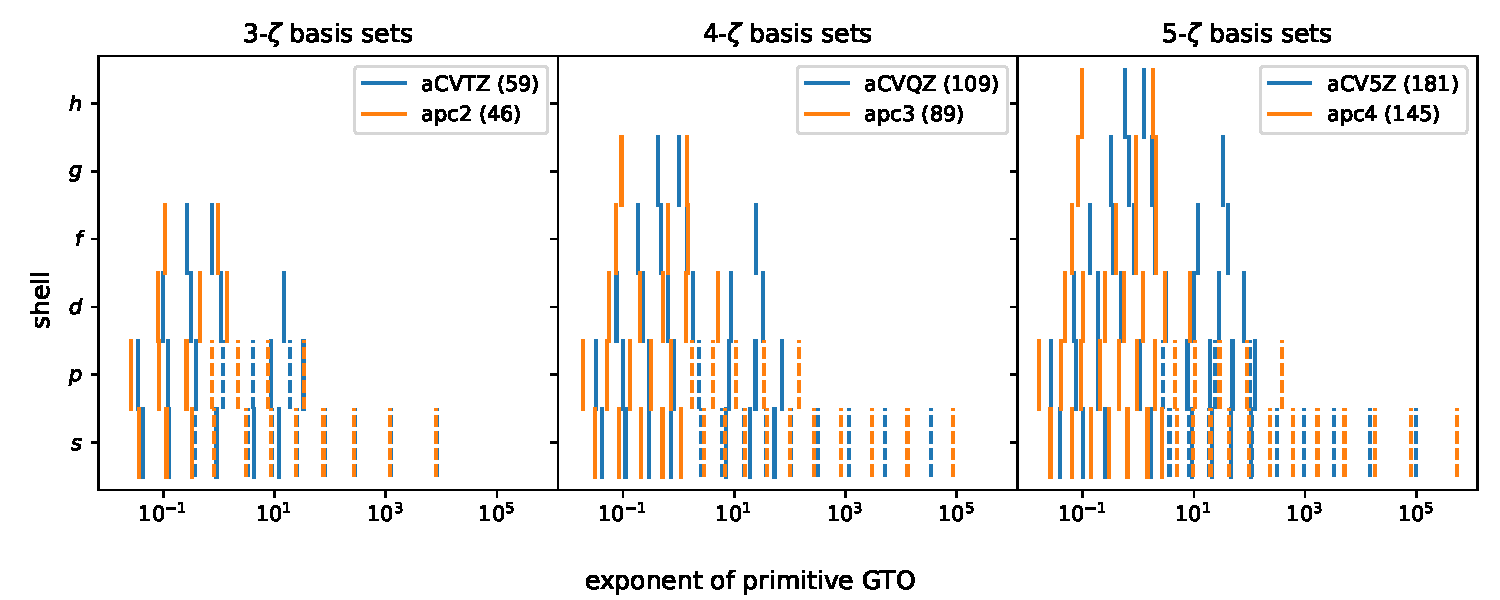
\includegraphics[width=0.9\textwidth]{assets/basis_exponent_plot.pdf}
    \caption{aCV$X$Z ($X=\mathrm{T,Q,5}$) 与 apc$n$ ($n=2,3,4$) 碳原子基函数构成。线条对应的横坐标是 GTO 的指数。实线对应的是作为基函数的原始 GTO。虚线对应的是 CGTO 中被缩并的原始 GTO;单根虚线不构成基。缩并系数信息未展示于该图。图例括号中的数字代表该基组碳原子的基函数数量。}
    \label{fig.6.basis-exponent-plot}
\end{figure}

当对比 apc$n$ ($n=2,3,4$) 与 aCV5Z 时,如图 \ref{fig.6.basis-exponent-plot-compare} 所示,可以发现每个壳层下,apc$n$ 基组的弥散函数普遍比 aCV5Z 更加弥散 (除了 apc2 在 $d$ 壳层的弥散基组)。aCV5Z 相对于 apc$n$ 来说,则是增加了靠近原子核区域的原始 GTO 基函数、以及在价层区域有更为密集的原始 GTO 基函数。

\begin{figure}[!ht]
    \centering
    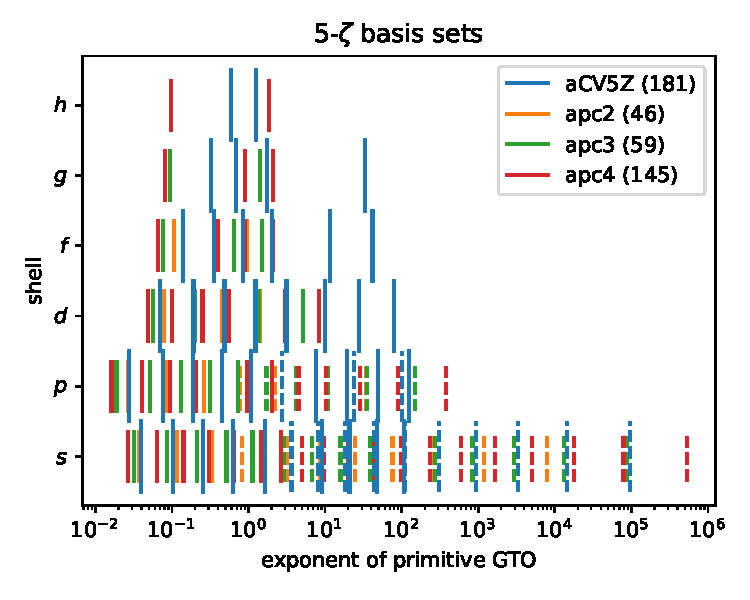
\includegraphics[width=0.4\textwidth]{assets/basis_exponent_plot_compare.pdf}
    \caption{aCV5Z 与 apc$n$ ($n=2,3,4$) 碳原子基函数构成。图例参考图 \ref{fig.6.basis-exponent-plot}。}
    \label{fig.6.basis-exponent-plot-compare}
\end{figure}

\subsubsection{B2PLYP 同性极化率中自洽场泛函部分 $\alpha_\textsf{SCF}$ 的收敛趋势}

这一小节中,为简化分析,我们仅细致考察同性极化率 $\alpha$ 的基组收敛趋势。接续 \ref{sec.6.basis-converg} 节的做法,作为双杂化的典型泛函的典型,我们对 B2PLYP 的基组收敛趋势作详细分析。由于自洽场部分 $\alpha_\textsf{SCF}$ 与微扰部分 $\symup{\Delta} \alpha_\textsf{PT2}$ 的收敛趋势并不相同,因此两个贡献部分将分开讨论。

这里的分析将使用小提琴图 (violin plot)。该图像的纵坐标轴是双对数 (symmetric logarithmic) 缩放,线性区间为 $-0.01$\% 至 $0.01$\%;图像的数据密度建模方式是 Gaussian 核,采样的数据是纵坐标轴缩放后的结果 (而非误差本身),模型参数设为较小的 \texttt{bw\_method=0.1}。图像纵坐标的主格点是 $\pm 10^{n} \%$ $(n = -2, -1, 0, 1)$,副格点是 $\pm 5 \times 10^{n} \%$ $(n = -2, -1, 0)$。该类型图可以展示数据分布的细节,但当前的绘制方式不会凸显较为异常的数值;相对地,正文中的相对方均根误差 RelRMSD 对误差较大的数据比较敏感,两种分析可以互补。同时,小提琴图展示的是误差分布本身,而非每个数据点的误差随着基组增大而变化的趋势;因此仍然无法分析具体分子或某一类分子的基组收敛趋势。

\begin{figure}[!ht]
    \centering
    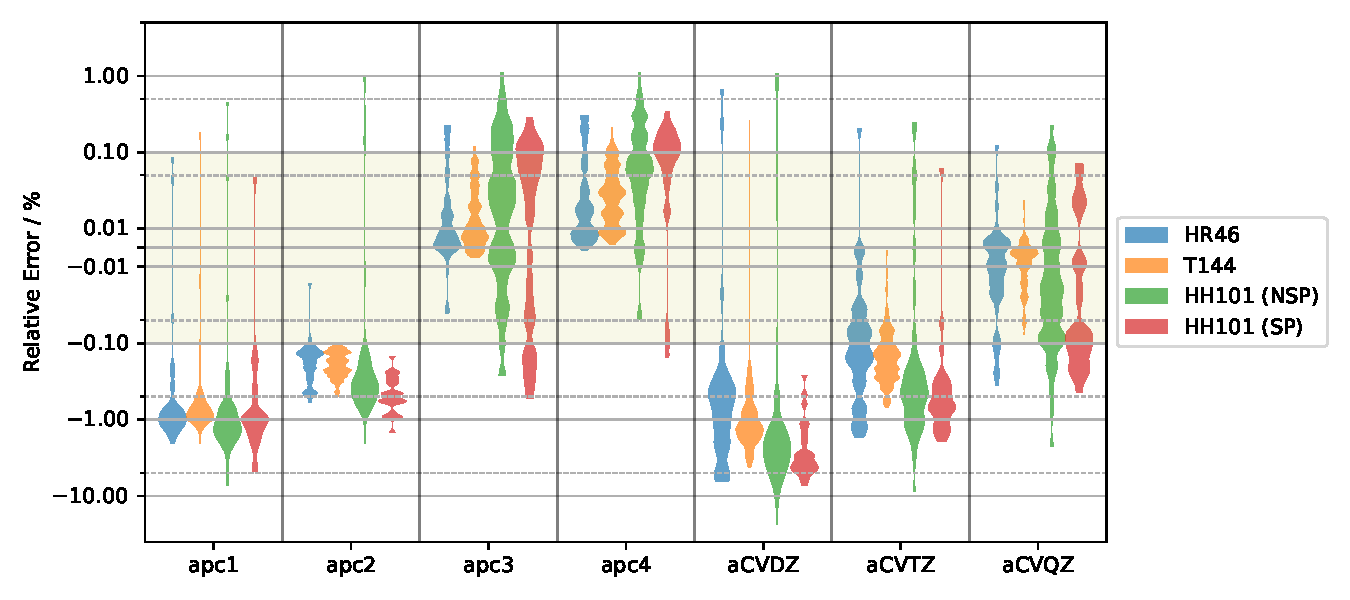
\includegraphics[width=0.9\textwidth]{assets/converg-b2p-scf-aCV5Z.pdf}
    \caption{B2PLYP 同性极化率的自洽场贡献部分 $\alpha_\textsf{SCF}$ 不同基组相对于 aCV5Z 的相对误差。对于 HH101 非自旋极化数据集 (NSP),氢原子未纳入该图的分析 (下同)。}
    \label{fig.6.converg-b2p-scf-aCV5Z}
\end{figure}

图 \ref{fig.6.converg-b2p-scf-aCV5Z} 展示的是当选取 aCV5Z 基组作为参考值时,B2PLYP 自洽场部分同性极化率 $\alpha_\textsf{SCF}$ 在不同基组下的相对误差。总体来说,基组越大,误差分布大体上越接近零点附近;这意味着 aCV5Z 基组确实比较接近基组极限,以及 aCV$X$Z 与 apc$n$ 基组随着基数增大有较好的收敛性。

但同时注意到,一方面,$\alpha_\textsf{SCF}$ 一般随着基组增大,其数值也相应地增大;反映在误差表现上,则是相对误差随基组增大而愈加趋近正值;就此我们推测,对于当前工作所测评的大多数分子,分子的极化率随着基组接近基组极限而增大。我们认为,Brakestad 等人工作\cite{Brakestad-Frediani.JCTC.2020} Figure 6 数据表现也支持这个观点:尽管这并非 Brakestad 等人原文的结论,但可以发现在 PBE 泛函下 apc4 相比于更为精确的 MW7 基组的误差大体上是负误差\footnote{通过对 Brakestad 等人工作\cite{Brakestad-Frediani.JCTC.2020} 的 Supporting Information 分析,可以发现对于 PBE 泛函下 apc4 解析极化率与 MW7 数值极化率的相对误差,其所测评的 124 个体系 (HH132 数据集排除了 8 个分子),除了 \ce{^2HO2} 与 \ce{^2Na} 两个奇异情形外,其余体系的平均误差是 $-0.025\%$、方均根误差是 $0.061\%$。误差大于 $0.1\%$ 的体系共 2 个 (\ce{Mg}, \ce{^2SF},其中 $\ce{^2SF}$ 在我们的工作中不作测评)、大于 $0.01\%$ 的体系共 7 个;误差小于 $-0.1\%$ 的体系共 8 个 (\ce{^2H2O-Li}, \ce{Na2}, \ce{Li}, \ce{He}, \ce{Ne}, \ce{NaLi}, \ce{^2BeH}, \ce{Ar},其中 \ce{Na2} 在我们的工作中不测评)。Brakestad 等人工作中分子 \ce{^2HO2} 与 \ce{^2Na} 的 PBE 泛函 apc4 解析极化率与 MW7 数值极化率误差大于 0.9\%;在我们的工作中,这两个分子的 B2PLYP 自洽场部分 apc4 与 aCV5Z 极化率之间相对误差较小 (分别为 0.199\% 与 -0.154\%),二阶微扰部分 \ce{^2HO2} 误差很小 (0.025\%)、\ce{^2Na} 误差较大 (0.453\%)}。

另一方面,对比 apc3 和 apc4 相对于 aCV5Z 基组的误差,我们发现对于所有被测评的数据集,绝大多数分子的 apc4 误差都大于零;而 apc3 作为更小的基组,尽管有更广的误差分布,但更多分子的误差反而更接近于零;这照应了正文的表 \ref{tab.6.b2p-conv-hr46-t144-iso} 的 HR46 与 T144 数据集、与表 \ref{tab.6.b2p-conv-hh101-iso} 的 HH101 (NSP) 数据集中,apc4 的 $\alpha_\textsf{SCF}$ RelRMSD 误差比 apc3 更大的结论;而若参考值足够准确,这样的结论是较为反常的。

综合上述推测与数据表现,我们猜测 apc4 尽管基函数数量更少,但在计算 $\alpha_\textsf{SCF}$ 的问题上很可能比 aCV5Z 更接近基组极限。若将 $\alpha_\textsf{SCF}$ 参考值设定为 apc4,如图 \ref{fig.6.converg-b2p-scf-apc4} 所示,则不论是 apc$n$ ($n=1,2,3$) 或 aCV$X$Z ($X = \mathrm{[D,T,Q,5]}$),绝大多数分子的误差均是负误差;且对于同系列基组,误差趋势随基组基数的增大而稳定地减少。结合对图 \ref{fig.6.basis-exponent-plot} 与图 \ref{fig.6.basis-exponent-plot-compare} 附近的讨论,我们认为这有可能与 apc4 弥散基组的原始 GTO 基函数指数较小、相比于 aCV5Z 更为弥散有关。

\begin{figure}[!ht]
    \centering
    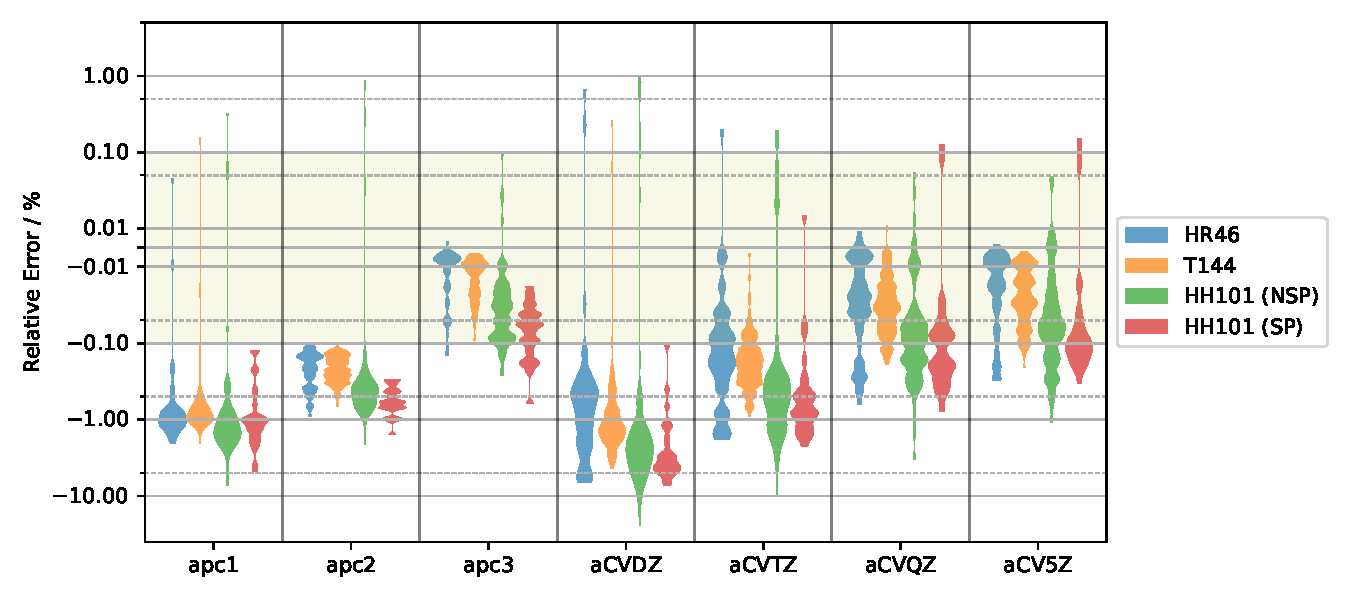
\includegraphics[width=0.9\textwidth]{assets/converg-b2p-scf-apc4.pdf}
    \caption{B2PLYP 同性极化率的自洽场贡献部分 $\alpha_\textsf{SCF}$ 不同基组相对于 apc4 的相对误差。}
    \label{fig.6.converg-b2p-scf-apc4}
\end{figure}

\subsubsection{B2PLYP 同性极化率二阶微扰部分 $\symup{\Delta} \alpha_\textsf{PT2}$ 的收敛趋势}

图 \ref{fig.6.converg-b2p-pt2-aCV5Z} 与图 \ref{fig.6.converg-b2p-pt2-apc4} 分别展示了以 aCV[Q5]Z 与 apc[34] 作为参考值下 $\symup{\Delta} \alpha_\textsf{PT2}$ 的相对误差收敛趋势。首先,从收敛趋势上,除了 aCVDZ 基组或 HH101 的自旋极化分子集,其余情形绝大多数分子的误差是正误差、且误差确实随基组基数的增大而逐步地逼近零。这表明以 aCV[Q5]Z 与 apc[34] 这两种 CBS 外推模型作为参考值,都有较好的基组收敛性趋势。

\begin{figure}[!ht]
    \centering
    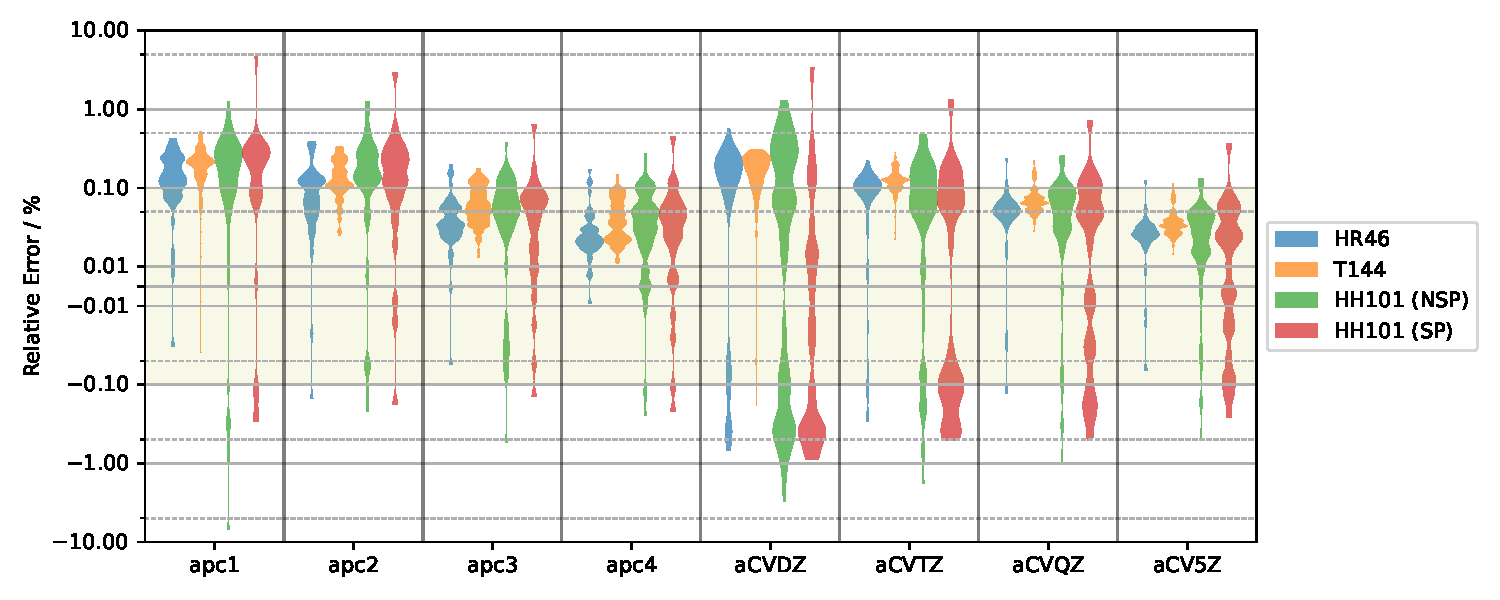
\includegraphics[width=0.9\textwidth]{assets/converg-b2p-pt2-aCV5Z.pdf}
    \caption{B2PLYP 同性极化率的自洽场贡献部分 $\symup{\Delta} \alpha_\textsf{PT2}$ 不同基组相对于 aCV[Q5]Z 的相对误差。}
    \label{fig.6.converg-b2p-pt2-aCV5Z}
\end{figure}

\begin{figure}[!ht]
    \centering
    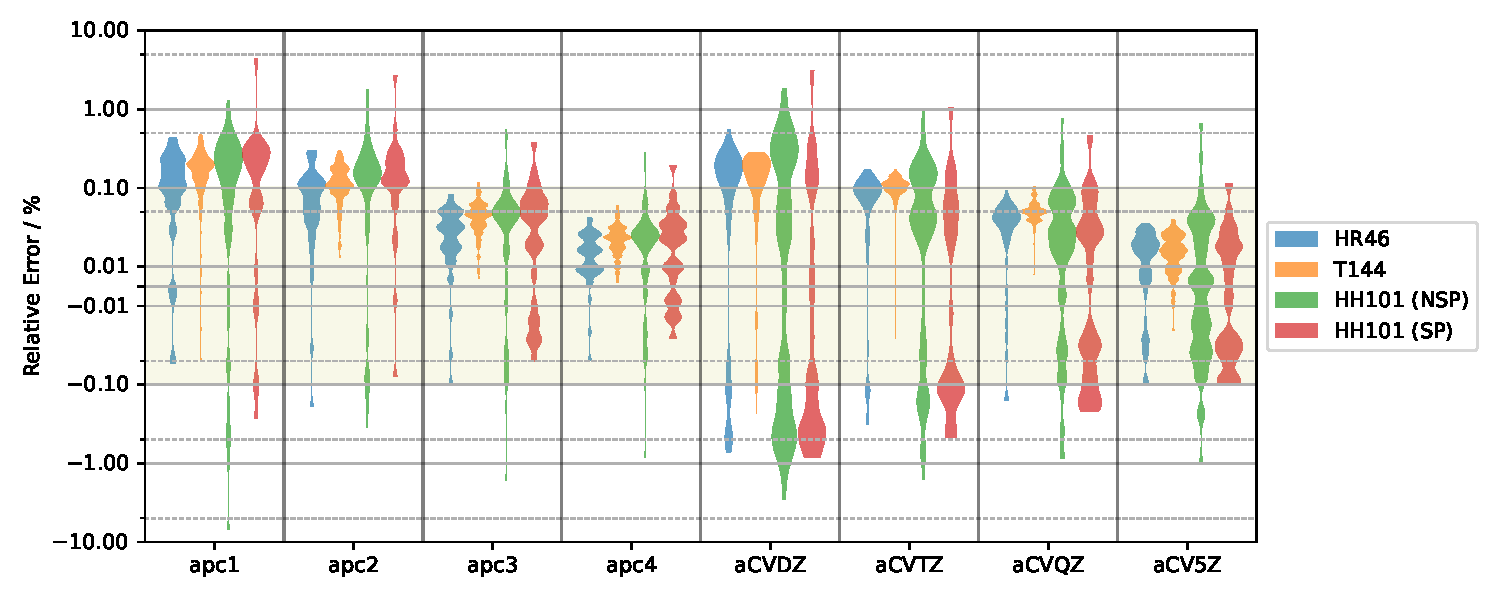
\includegraphics[width=0.9\textwidth]{assets/converg-b2p-pt2-apc4.pdf}
    \caption{B2PLYP 同性极化率的自洽场贡献部分 $\symup{\Delta} \alpha_\textsf{PT2}$ 不同基组相对于 apc[34] 的相对误差。}
    \label{fig.6.converg-b2p-pt2-apc4}
\end{figure}

但相比于 PBE 泛函可以通过极高精度的 MW7 基组实现 $\alpha_\textsf{SCF}$ 的计算,目前更高基组精度的 $\symup{\Delta} \alpha_\textsf{PT2}$ 计算较为困难;也鲜有在 $\symup{\Delta} \alpha_\textsf{PT2}$ 计算问题上广受验证与测试的高精度 CBS 外推模型\footnote{CBS 外推方法最初是针对相关能而设计的计算方法\cite{Nyden-Petersson.JCP.1981};尽管 CBS 外推方法有长足的发展\cite{Peterson-Dunning.JCP.1994, Nyden-Petersson.JCP.1981, Petersson-Mantzaris.JCP.1988, Jensen-Jensen.TCA.2005, Karton-Martin.TCA.2006, Klopper-Kutzelnigg.JMST.1986, Kutzelnigg-Morgan.JCP.1992, Martin-Martin.CPL.1996, Helgaker-Noga.JCP.1997, Halkier-Wilson.CPL.1998, Halkier-Olsen.CPL.1999},但这些发展通常仍然是提升能量的描述精度。而对于性质的计算,则通常使用与能量计算相同的 CBS 外推模型\cite{Monten-Deleuze.MP.2011, Huzak-Deleuze.JCP.2013, Hait-Head-Gordon.JCTC.2018, Hait-Head-Gordon.PCCP.2018},而鲜有专门针对性质本身设计的 CBS 外推模型。}。同时与 $\alpha_\textsf{SCF}$ 的分析不同,即当使用 apc4 作为 $\alpha_\textsf{SCF}$ 参考值时,基组随基数增大而收敛的趋势比使用 aCV5Z 作为参考值的情形要更加明朗清晰;对于 $\symup{\Delta} \alpha_\textsf{PT2}$,不论使用 aCV[Q5]Z 或 apc[34] 基组的收敛趋势都较为正常。因此,依现有的数据,我们无法判断何种 CBS 外推模型更接近基组极限。

\subsubsection{BSIE 误差的推测}

在正文的工作中,我们主要使用 apc3 基组进行测评计算。在没有基组极限结果的情况下,对于同性极化率 $\alpha_\textsf{DH} = \alpha_\textsf{SCF} + \symup{\Delta} \alpha_\textsf{PT2}$ 的计算,其 BSIE 误差的来源在于
\begin{itemize}[nosep]
    \item 分析基组收敛性时,作为参考值的基组 (5-$\zeta$ 的基组或 CBS 外推模型) 本身的误差;
    \item apc3 与参考值之间的误差。
\end{itemize}

\begin{table}[!ht]
\centering
\caption{B2PLYP 泛函 apc[34] 与 aCV[Q5]Z 外推模型间同性极化率 $\alpha$ 的基组相对方均根误差 (RelRMSD / \%)。}
\label{tab.6.b2p-conv-5zeta}
\widetabular{
    \begin{tabular}{ld{2.4}d{2.4}d{2.4}}
    \toprule
    dataset                & \multicolumn{1}{c}{$\tilde \alpha_\textsf{SCF}$\tnote{b}} & \multicolumn{1}{c}{$\symup{\Delta} \tilde \alpha_\textsf{PT2}$\tnote{c}} & \multicolumn{1}{c}{$\tilde \alpha_\textsf{DH}$\tnote{d}} \\ \midrule
    HR46                   & 0.099 & 0.034 & 0.127 \\
    T144                   & 0.050 & 0.032 & 0.080 \\
    HH101 (NSP)\tnote{a} & 0.214 & 0.154 & 0.282 \\
    HH101 (SP)             & 0.135 & 0.094 & 0.177 \\ \bottomrule
    \end{tabular}
}{
    \item[a] 该误差数据未将氢原子体系纳入统计,即总共分析了 74 个 HH101 数据集的自旋非极化分子体系。
    \item[b] $\text{RelRMSD} (\tilde \alpha_{\textsf{SCF}/\text{apc4}}, \tilde \alpha_{\textsf{SCF}/\text{aCV5Z}}, \tilde \alpha_{\textsf{DH}/\text{aCV[Q5]Z}})$。
    \item[c] $\text{RelRMSD} (\symup{\Delta} \tilde \alpha_{\textsf{PT2}/\text{apc[34]}}, \symup{\Delta} \tilde \alpha_{\textsf{PT2}/\text{aCV[Q5]Z}}, \tilde \alpha_{\textsf{DH}/\text{aCV[Q5]Z}})$。
    \item[d] $\text{RelRMSD} (\tilde \alpha_{\textsf{DH}/\text{apc[34]}}, \tilde \alpha_{\textsf{DH}/\text{aCV[Q5]Z}})$。
}
\end{table}

表 \ref{tab.6.b2p-conv-5zeta} 的数据总结了两种 5-$\zeta$ 级别 CBS 外推模型 apc[34] 与 aCV[Q5]Z 之间的相对误差。首先,对于 $\alpha_\textsf{SCF}$ 的误差,可以看到 HH101 数据集的误差显著地大于 HR46 与 T144 数据集。而 Brakestad 等人工作\cite{Brakestad-Frediani.JCTC.2020}中对 PBE 泛函的误差分析表明,除去两个奇异分子 \ce{^2HO2} 与 \ce{^2Na},其所测评的 HH132 数据集中的 122 个体系 apc4 基组相对于非常接近基组极限的 MW7 基组的相对方均根误差是 0.061\%;远小于我们工作中 B2PLYP 自洽场部分 apc4 与 aCV5Z 之间的 0.214\% (自旋非极化体系) 或 0.135\% (自旋极化体系) 的误差。在假定 B2PLYP 的自洽场部分基组收敛性与 PBE 较为接近的前提下,我们倾向于认为作为 HH132 数据集的子集,HH101 数据集 $\alpha_\textsf{SCF}$ 在 apc4 基组下的相对 BSIE 在 0.06\% 左右;而对于 HR46 与 T144 数据集,apc4 的相对 BSIE 可能更低。对于 $\symup{\Delta} \alpha_\textsf{PT2}$,在没有更精确的基组作为参考值的情况下,我们通过 apc[34] 与 aCV[Q5]Z 之间的相对误差来估计相对 BSIE 大小。对于 HH101 数据集的非自旋极化体系,该相对误差是 0.154\%;其他数据集的相对误差更小。综上,在所测评的数据集、以及 apc[34] 外推模型下,我们预估 B2PLYP 同性极化率 $\tilde \alpha_\textsf{DH}$ 相对 BSIE 将不大于 0.2\%。

\begin{table}[!ht]
\centering
\caption{B2PLYP apc3 与 apc[34] 间极化率的基组相对方均根误差 (RelRMSD / \%)。}
\label{tab.6.b2p-conv-apc3}
\widetabular{
    \begin{tabular}{lld{2.4}d{2.4}d{2.4}}
    \toprule
    性质 & 数据集 & \multicolumn{1}{c}{SCF} & \multicolumn{1}{c}{PT2} & \multicolumn{1}{c}{DH} \\ \midrule
    同性极化率\tnote{a}     & HR46                   & 0.041 & 0.039            & 0.035 \\
    & T144                   & 0.024 & 0.050            &0.032 \\
    & HH101 (NSP)\tnote{d} & 0.074 & 0.218\tnote{e} & 0222 \\
    & HH101 (SP)             & 0.159\tnote{f} & 0.095 & 0.145 \\ \midrule
    异性极化率\tnote{b}   & HR46                   & 0.046 & 0.152\tnote{g} & 0.167 \\
    & T144                   & 0.018 & 0.061            & 0.070 \\ \midrule
    极化率分量\tnote{c}    & HH101 (NSP)\tnote{d} & 0.081 & 0.353\tnote{h} & 0.355 \\
    & HH101 (SP)             & 0.165\tnote{i} & 0.101 & 0.153 \\ \bottomrule
    \end{tabular}
}{
    \item[a] 这部分测评的是同性极化率 $\tilde \alpha_\textsf{SCF}, \symup{\Delta} \tilde \alpha_\textsf{PT2}, \tilde \alpha_\textsf{DH}$ 的误差;RelRMSD 误差的具体定义参考表 \ref{tab.6.b2p-conv-hr46-t144-iso} 表头的注释,作为参考值的基组为 apc[34]。
    \item[b] 这部分测评的是异性极化率 $\tilde \gamma_\textsf{SCF}, \symup{\Delta} \tilde \gamma_\textsf{PT2}, \tilde \gamma_\textsf{DH}$ 的误差;RelRMSD 误差的具体定义参考表 \ref{tab.6.b2p-conv-hr46-t144-aniso} 表头的注释,作为参考值的基组为 apc[34]。
    \item[c] 这部分测评的是极化率分量 $\alpha_{xx}, \alpha_{yy}, \alpha_{zz}$ 在自洽场部分、二阶微扰部分、与总和的误差;RelRMSD 误差的具体定义参考表 \ref{tab.6.b2p-conv-hh101-rmsre} 表头的注释,作为参考值的基组为 apc[34]。
    \item[d] 该误差数据未将氢原子体系纳入统计,即总共分析了 74 个 HH101 数据集的自旋非极化分子体系。
    \item[e] \ce{NaCl} 误差为 $-1.660\%$;去除该体系,误差将是 0.102\%。
    \item[f] \ce{^4P} 误差为 $-0.615\%$;去除该体系,误差将是 0.105\%。
    \item[g] \ce{N(CH3)3} 误差为 $-0.622\%$;去除该体系,误差将是 0.117\%。
    \item[h] 去除 \ce{NaCl},误差将是 0.110\%。
    \item[i] 去除 \ce{^4P},误差将是 0.103\%。
}
\end{table}

表 \ref{tab.6.b2p-conv-apc3} 的数据表明,除了一些特例分子 (包括 \ce{NaCl}, \ce{N(CH3)3}, \ce{^4P}),其余情形下 apc3 基组相对于 apc[34],自洽场与二阶微扰两个贡献量的相对误差均不大于 0.1\%;因此,总极化率作为自洽场与二阶微扰贡献量之和,误差不超过 0.2\%。结合上一段的分析,我们认为对于绝大多数分子,apc3 的 BSIE 误差应不大于 0.4\%,处在实验误差 0.5\% 范围以内。

作为这一小节的总结,我们首先注意到了正文的基组收敛性分析中,以 aCV[Q5]Z 为参考值时,以表 \ref{tab.6.b2p-conv-hr46-t144-iso} 为代表的一些测评基准下,存在 apc4 相较于 apc3 误差更大的情形;同时注意到 Brakestad 等人工作\cite{Brakestad-Frediani.JCTC.2020}表明 apc4 的 BSIE 误差相当小,因而引起了我们对 aCV[Q5]Z 作为参考值准确性的疑问、并且希望对 5-$\zeta$ 级别基组或 CBS 外推方法 BSIE 误差作分析。我们从基组的原始 GTO 基函数指数大小、同性极化率误差分布的基组收敛性、以及对比 Brakestad 等人工作\cite{Brakestad-Frediani.JCTC.2020}的结果入手,推断 apc4 相较于 aCV5Z 在 $\alpha_\textsf{SCF}$ 的计算问题上可能具有更低的 BSIE。对于 B2PLYP 泛函,以 apc[34] 作为参考值、并且引入 apc[34] 外推模型的 BSIE 预估值,我们认为绝大多数分子的 apc3 的 BSIE 误差不超过 0.4\%。这与正文中以 aCV[Q5]Z 作为参考值、且未引入 aCV[Q5]Z 的 BSIE 预估值的误差分析结论相仿;因此,使用 apc3 作为双杂化泛函静态极化率的测评基组是合理的。

\subsection{其他补充数据}

\begin{itemize}[nosep]
    \item 表 \ref{tab.6.full-benchmark} 展示了所有经测评密度泛函近似的极化率误差表现。
\end{itemize}

\newpage

\begingroup
\setlength{\LTleft}{-20cm plus -1fill}
\setlength{\LTright}{\LTleft}

\begin{landscape}
\begin{longtable}[c]{lcccccrrrrrrrrc}
\caption{诸密度泛函近似在数据集 HR46、T144 与 HH101 上的极化率测评表现。除 WTRE 为无量纲量外,其余误差以 RelRMSD (\%) 计算${}^a$。}
\label{tab.6.full-benchmark}
\\ \toprule
& & & \multicolumn{3}{c}{杂化类型} & \multicolumn{4}{c}{同性极化率} & \multicolumn{2}{c}{异性极化率} & \multicolumn{2}{c}{极化率分量} & \\
\cmidrule(lr){4-6} \cmidrule(lr){7-10} \cmidrule(lr){11-12} \cmidrule(lr){13-14}
计算方法 & 年代 & 组成 & 交换\tabnote{b} & 相关\tabnote{c} & xDH & \multicolumn{1}{c}{HR46} & \multicolumn{1}{c}{T144} & \multicolumn{2}{c}{HH101} & \multicolumn{1}{c}{HR46} & \multicolumn{1}{c}{T144} & \multicolumn{2}{c}{HH101} & \multicolumn{1}{c}{WTRE} \\
\cmidrule(lr){9-10} \cmidrule(lr){13-14}
& & & & & & & & \multicolumn{1}{c}{NSP} & \multicolumn{1}{c}{SP} & & & \multicolumn{1}{c}{NSP} & \multicolumn{1}{c}{SP} & \\ \midrule
\endfirsthead
\caption{(续表)}
\\ \toprule
& & & \multicolumn{3}{c}{杂化类型} & \multicolumn{4}{c}{同性极化率} & \multicolumn{2}{c}{异性极化率} & \multicolumn{2}{c}{极化率分量} & \\
\cmidrule(lr){4-6} \cmidrule(lr){7-10} \cmidrule(lr){11-12} \cmidrule(lr){13-14}
计算方法 & 年代 & 组成 & 交换\tabnote{b} & 相关\tabnote{c} & xDH & \multicolumn{1}{c}{HR46} & \multicolumn{1}{c}{T144} & \multicolumn{2}{c}{HH101} & \multicolumn{1}{c}{HR46} & \multicolumn{1}{c}{T144} & \multicolumn{2}{c}{HH101} & \multicolumn{1}{c}{WTRE} \\
\cmidrule(lr){9-10} \cmidrule(lr){13-14}
& & & & & & & & \multicolumn{1}{c}{NSP} & \multicolumn{1}{c}{SP} & & & \multicolumn{1}{c}{NSP} & \multicolumn{1}{c}{SP} & \\ \midrule
\endhead
\bottomrule
\endfoot
%
XYGJ-OS          & 2011 & GGA  & hyb & hyb & xDH & 0.911 & 0.813 & 1.235  & 1.592  & 2.756  & 1.845  & 1.381  & 1.762  & 0.418 \\
XYG6             & 2021 & GGA  & hyb & hyb & xDH & 1.040 & 1.050 & 1.285  & 1.905  & 2.841  & 2.112  & 1.429  & 2.101  & 0.472 \\
CCSD             &      & WFT  &     &     &     & 1.294 & 1.567 & 1.507  & 1.141  & 2.372  & 2.313  & 1.556  & 1.283  & 0.473 \\
DSD-PBEPBE-D3BJ  & 2013 & GGA  & hyb & hyb &     & 1.146 & 1.274 & 1.615  & 1.412  & 2.234  & 2.446  & 1.651  & 1.578  & 0.473 \\
xDH-PBE0         & 2012 & GGA  & hyb & hyb & xDH & 0.685 & 0.561 & 2.014  & 2.216  & 2.554  & 1.648  & 2.049  & 2.439  & 0.476 \\
XYG-OS5          & 2021 & GGA  & hyb & hyb & xDH & 0.817 & 0.625 & 1.477  & 2.200  & 3.678  & 2.096  & 1.636  & 2.368  & 0.488 \\
ωPBEPP86         & 2021 & GGA  & rsh & hyb &     & 1.093 & 1.069 & 2.068  & 0.949  & 3.252  & 2.542  & 2.090  & 1.074  & 0.490 \\
XYG5             & 2021 & GGA  & hyb & hyb & xDH & 1.095 & 1.138 & 1.330  & 1.981  & 2.739  & 2.235  & 1.479  & 2.197  & 0.490 \\
revXYGJ-OS       & 2021 & GGA  & hyb & hyb & xDH & 0.965 & 0.680 & 1.515  & 2.187  & 3.624  & 2.025  & 1.716  & 2.384  & 0.501 \\
XYG3             & 2009 & GGA  & hyb & hyb & xDH & 1.083 & 1.385 & 1.345  & 2.047  & 2.513  & 3.141  & 1.456  & 2.272  & 0.524 \\
revXYG3          & 2021 & GGA  & hyb & hyb & xDH & 0.971 & 1.062 & 1.739  & 2.410  & 2.493  & 2.671  & 1.858  & 2.645  & 0.540 \\
ωB88PP86         & 2021 & GGA  & rsh & hyb &     & 1.434 & 1.490 & 2.225  & 1.130  & 2.978  & 2.817  & 2.270  & 1.273  & 0.559 \\
ωB2GP-PLYP       & 2019 & GGA  & rsh & hyb &     & 1.062 & 1.140 & 2.374  & 1.829  & 3.005  & 2.824  & 2.403  & 1.875  & 0.569 \\
DSD-PBEP86-D3BJ  & 2013 & GGA  & hyb & hyb &     & 1.720 & 1.826 & 1.974  & 1.317  & 2.563  & 2.714  & 2.032  & 1.420  & 0.574 \\
PBE-QIDH         & 2014 & GGA  & hyb & hyb &     & 1.026 & 1.160 & 2.252  & 1.775  & 3.478  & 3.275  & 2.268  & 1.983  & 0.582 \\
DSD-BLYP-D3BJ    & 2013 & GGA  & hyb & hyb &     & 1.552 & 1.709 & 1.865  & 1.776  & 3.022  & 2.977  & 1.919  & 1.907  & 0.596 \\
SOS0-PBE-QIDH    & 2016 & GGA  & hyb & hyb &     & 1.147 & 1.209 & 2.216  & 2.188  & 3.243  & 2.665  & 2.241  & 2.489  & 0.598 \\
XYG7             & 2021 & GGA  & hyb & hyb & xDH & 2.003 & 1.947 & 2.029  & 1.575  & 2.767  & 2.111  & 2.097  & 1.758  & 0.611 \\
PBE0-2           & 2012 & GGA  & hyb & hyb &     & 1.040 & 0.850 & 2.189  & 3.393  & 3.306  & 2.334  & 2.193  & 3.695  & 0.637 \\
lrc-XYG3         & 2013 & GGA  & hyb & rsh & xDH & 1.294 & 1.733 & 2.405  & 2.020  & 2.799  & 3.565  & 2.479  & 2.260  & 0.651 \\
ωB2PLYP          & 2019 & GGA  & rsh & hyb &     & 1.217 & 1.314 & 2.691  & 2.362  & 3.170  & 3.122  & 2.729  & 2.392  & 0.656 \\
PBE-CIDH         & 2015 & GGA  & hyb & hyb &     & 1.101 & 1.564 & 2.182  & 2.100  & 4.310  & 4.500  & 2.214  & 2.216  & 0.673 \\
RS-B88-LYP       & 2021 & GGA  & rsh & rsh &     & 1.149 & 0.860 & 2.603  & 3.622  & 2.894  & 2.010  & 2.616  & 4.145  & 0.679 \\
LS1DH-PBE        & 2011 & GGA  & hyb & hyb &     & 1.012 & 0.989 & 2.229  & 3.833  & 3.250  & 2.752  & 2.238  & 4.224  & 0.686 \\
B2GP-PLYP        & 2008 & GGA  & hyb & hyb &     & 1.680 & 1.987 & 2.004  & 2.254  & 3.254  & 3.747  & 2.071  & 2.396  & 0.686 \\
SOS0-PBE0-DH     & 2016 & GGA  & hyb & hyb &     & 1.111 & 1.587 & 2.146  & 2.320  & 4.332  & 4.470  & 2.188  & 2.442  & 0.686 \\
TPSS-QIDH        & 2014 & mGGA & hyb & hyb &     & 1.210 & 1.223 & 2.782  & 2.462  & 3.715  & 3.304  & 2.803  & 2.718  & 0.688 \\
RS-PBE-PBE       & 2021 & GGA  & rsh & rsh &     & 1.161 & 0.822 & 2.857  & 3.445  & 3.058  & 1.988  & 2.869  & 4.048  & 0.691 \\
RS-PBE-P86       & 2021 & GGA  & rsh & rsh &     & 1.160 & 0.819 & 2.906  & 3.491  & 3.100  & 2.002  & 2.918  & 4.073  & 0.698 \\
ωB97X-2-TQZ      & 2009 & GGA  & rsh & hyb &     & 1.732 & 1.769 & 2.785  & 2.196  & 2.943  & 2.394  & 2.836  & 2.641  & 0.699 \\
RS-PW91-PW91     & 2021 & GGA  & rsh & rsh &     & 1.223 & 0.853 & 2.937  & 3.474  & 3.094  & 1.986  & 2.950  & 4.080  & 0.706 \\
PBE0-DH          & 2011 & GGA  & hyb & hyb &     & 1.173 & 1.730 & 2.213  & 2.286  & 4.607  & 4.925  & 2.251  & 2.375  & 0.718 \\
PTPSS-D3Zero     & 2011 & mGGA & hyb & hyb &     & 1.823 & 2.138 & 2.385  & 2.477  & 3.131  & 4.104  & 2.450  & 2.530  & 0.749 \\
RSX-QIDH         & 2018 & GGA  & rsh & hyb &     & 1.530 & 1.584 & 3.278  & 2.226  & 4.044  & 3.122  & 3.308  & 2.879  & 0.766 \\
revPBE0-DH       & 2013 & GGA  & hyb & hyb &     & 1.165 & 1.759 & 2.322  & 2.936  & 4.701  & 4.978  & 2.363  & 3.070  & 0.773 \\
TPSS-CIDH        & 2015 & mGGA & hyb & hyb &     & 1.238 & 1.548 & 2.782  & 2.889  & 4.646  & 4.503  & 2.849  & 3.125  & 0.789 \\
TPSS0-DH         & 2013 & mGGA & hyb & hyb &     & 1.241 & 1.662 & 2.760  & 3.028  & 4.953  & 4.910  & 2.805  & 3.252  & 0.819 \\
SOS-RSX-PBE-QIDH & 2021 & GGA  & rsh & hyb &     & 1.821 & 1.933 & 3.331  & 2.662  & 4.408  & 3.197  & 3.370  & 3.398  & 0.848 \\
MPW1K            & 2000 & GGA  & hyb &     &     & 1.654 & 2.024 & 2.899  & 2.426  & 5.929  & 5.502  & 2.971  & 2.663  & 0.877 \\
mPW2PLYP         & 2006 & GGA  & hyb & hyb &     & 2.255 & 2.678 & 2.647  & 3.273  & 3.948  & 4.853  & 2.762  & 3.431  & 0.918 \\
SCAN0            & 2016 & mGGA & hyb &     &     & 1.718 & 2.551 & 2.504  & 2.668  & 6.328  & 7.160  & 2.608  & 2.857  & 0.946 \\
RSX-0DH          & 2019 & GGA  & rsh & hyb &     & 2.047 & 2.251 & 3.968  & 2.683  & 5.429  & 4.062  & 4.017  & 3.531  & 0.979 \\
PBE50            & 2012 & GGA  & hyb &     &     & 2.108 & 2.226 & 3.398  & 2.839  & 6.371  & 5.224  & 3.475  & 3.114  & 0.985 \\
MP2              &      & WFT  &     &     &     & 2.609 & 0.813 & 2.146  & 4.752  & 10.532 & 1.625  & 2.188  & 5.693  & 0.994 \\
B2PLYP           & 2006 & GGA  & hyb & hyb &     & 2.552 & 2.987 & 2.908  & 3.468  & 4.256  & 5.194  & 2.998  & 3.656  & 1.002 \\
SOS-RSX-PBE0-DH  & 2021 & GGA  & rsh & hyb &     & 2.188 & 2.401 & 4.005  & 2.850  & 5.618  & 4.096  & 4.058  & 3.737  & 1.016 \\
M11              & 2011 & mGGA & rsh &     &     & 1.490 & 1.859 & 4.525  & 4.341  & 5.459  & 5.046  & 4.682  & 5.799  & 1.117 \\
MVS              & 2015 & mGGA &     &     &     & 1.658 & 2.550 & 3.460  & 2.823  & 7.291  & 9.230  & 3.659  & 3.694  & 1.124 \\
CAM-B3LYP        & 2004 & GGA  & rsh &     &     & 2.315 & 2.612 & 4.080  & 4.621  & 4.286  & 5.258  & 4.184  & 4.733  & 1.127 \\
PBE0             & 1999 & GGA  & hyb &     &     & 2.478 & 3.247 & 3.874  & 4.148  & 6.272  & 7.493  & 3.979  & 4.243  & 1.232 \\
M06-2X           & 2006 & mGGA & hyb &     &     & 1.548 & 1.930 & 3.310  & 8.244  & 5.741  & 4.998  & 3.394  & 8.438  & 1.242 \\
MN15             & 2016 & mGGA & hyb &     &     & 2.613 & 2.892 & 3.366  & 7.328  & 4.785  & 6.037  & 3.500  & 7.908  & 1.324 \\
mBEEF            & 2014 & mGGA &     &     &     & 2.501 & 3.714 & 3.588  & 4.523  & 8.951  & 10.585 & 3.771  & 4.662  & 1.408 \\
M06              & 2006 & mGGA & hyb &     &     & 2.488 & 3.282 & 4.622  & 7.004  & 7.030  & 8.107  & 4.756  & 7.175  & 1.507 \\
ωB97M-V          & 2016 & mGGA & hyb &     &     & 3.188 & 3.207 & 5.395  & 8.415  & 4.615  & 4.898  & 5.555  & 8.627  & 1.555 \\
SCAN             & 2015 & mGGA &     &     &     & 3.410 & 4.485 & 4.688  & 4.841  & 8.410  & 10.529 & 4.792  & 5.153  & 1.597 \\
M06-L            & 2006 & mGGA &     &     &     & 1.847 & 3.131 & 3.835  & 9.348  & 7.531  & 9.761  & 4.118  & 9.793  & 1.614 \\
TPSSh            & 2003 & mGGA & hyb &     &     & 3.362 & 4.396 & 4.966  & 5.497  & 7.975  & 9.892  & 5.070  & 5.628  & 1.619 \\
B3LYP            & 1993 & GGA  & hyb &     &     & 3.790 & 4.524 & 5.195  & 6.111  & 6.646  & 8.458  & 5.381  & 6.369  & 1.647 \\
HF               &      & WFT  &     &     &     & 4.727 & 4.126 & 6.592  & 5.948  & 13.901 & 8.483  & 6.868  & 7.069  & 1.986 \\
TPSS             & 2003 & mGGA &     &     &     & 4.875 & 5.916 & 6.843  & 7.721  & 10.162 & 12.239 & 6.998  & 8.071  & 2.198 \\
N12              & 2012 & GGA  &     &     &     & 4.666 & 5.446 & 7.607  & 11.687 & 11.588 & 13.180 & 8.072  & 12.043 & 2.535 \\
MPW91            & 1998 & GGA  &     &     &     & 6.042 & 6.860 & 8.515  & 10.081 & 11.414 & 13.041 & 8.712  & 11.005 & 2.665 \\
PBE              & 1997 & GGA  &     &     &     & 6.690 & 7.369 & 9.403  & 11.117 & 12.088 & 13.202 & 9.652  & 12.131 & 2.890 \\
BLYP             & 1988 & GGA  &     &     &     & 7.446 & 8.153 & 10.425 & 12.666 & 12.103 & 13.292 & 10.752 & 13.838 & 3.164
\end{longtable}
\vspace{-1em}
\footnotesize
\par\noindent\emph{a} 该表格以 WTRE 数值排序。作为参考值的方法是 CCSD(T);如前文所述,HH101 参考值由 Hait 与 Head-Gordon 在 aCV[TQ]Z 或 aCV[Q5]Z 级别下给出\cite{Hait-Head-Gordon.PCCP.2018};HR46 与 T144 参考值由本论文第五章给出,为 FPA-aV[DT]Z、FPA-aV[TQ]Z 或 FPA-aV[Q5]Z 级别下给出。
\par\noindent\emph{b} “hyb”指交换能中掺杂部分非局域的严格交换能;“exact”指交换能全部为严格交换能;“rsh”指交换能包含长短程分离的非局域交换能,不论其是否包含非局域短程交换。该项若非空缺,则视为杂化泛函。
\par\noindent\emph{c} “hyb”指相关能中掺杂 MP2 型非局域相关能;“rsh”指相关能中掺杂长短程分离的 MP2 型非局域相关能。该项若非空缺,则视为双杂化泛函。
\end{landscape}

\endgroup
